%%
%% The original source files were:
%%
%% samples.dtx  (with options: `all,proceedings,bibtex,manuscript')
%% 
%% IMPORTANT NOTICE:
%% 
%% For the copyright see the source file.
%% 
%% Any modified versions of this file must be renamed
%% with new filenames distinct from sample-manuscript.tex.
%% 
%% For distribution of the original source see the terms
%% for copying and modification in the file samples.dtx.
%% 
%% This generated file may be distributed as long as the
%% original source files, as listed above, are part of the
%% same distribution. (The sources need not necessarily be
%% in the same archive or directory.)
%%
%%
%% Commands for TeXCount
%TC:macro \cite [option:text,text]
%TC:macro \citep [option:text,text]
%TC:macro \citet [option:text,text]
%TC:envir table 0 1
%TC:envir table* 0 1
%TC:envir tabular [ignore] word
%TC:envir displaymath 0 word
%TC:envir math 0 word
%TC:envir comment 0 0
%%
%% The first command in your LaTeX source must be the \documentclass
%% command.
%%
%% For submission and review of your manuscript please change the
%% command to \documentclass[manuscript, screen, review]{acmart}.
%%
%% When submitting camera ready or to TAPS, please change the command
%% to \documentclass[sigconf]{acmart} or whichever template is required
%% for your publication.
%%
%%
\documentclass[manuscript,screen,review]{acmart}


\usepackage{algorithm}
% Use algorithmicx + algpseudocode: provides \Require, \Ensure, \State, and \Comment
\usepackage{algorithmicx}
\usepackage{algpseudocode}
% Table cell helpers and a portable checkmark command
\usepackage{pifont}
\usepackage{makecell}
% Provide \checkmark using pifont to avoid loading amssymb (which conflicts with newtx)
\providecommand{\checkmark}{\ding{51}}
% Common table marks used in comparison tables
% \cmark: satisfied, \xmark: not satisfied, \omark: partially satisfied
\newcommand{\cmark}{\ding{51}}
\newcommand{\xmark}{\ding{55}}
\newcommand{\omark}{\(\circ\)}
% Support table notes inside tables
\usepackage{threeparttable}
% Provide compatibility shims for uppercase macros used in the document
% Some authors use \REQUIRE/\ENSURE/\UPON/\ENDUPON (uppercase) — map them to algpseudocode
\providecommand{\REQUIRE}[1]{\Require{#1}}
\providecommand{\ENSURE}[1]{\Ensure{#1}}
% \UPON{<cond>} will render as a bold 'Upon <cond>' state line inside algorithmic blocks
\providecommand{\UPON}[1]{\State\textbf{Upon}~#1}
\providecommand{\ENDUPON}{}
% Provide uppercase aliases commonly used in algorithm blocks
\providecommand{\STATE}{\State}
\providecommand{\COMMENT}[1]{\Comment{#1}}
% Map common uppercase algorithmic keywords to algorithmicx/algpseudocode commands
\providecommand{\IF}{\If}
\providecommand{\ELSE}{\Else}
\providecommand{\ELSIF}{\ElsIf}
\providecommand{\ENDIF}{\EndIf}
\providecommand{\FOR}{\For}
\providecommand{\ENDFOR}{\EndFor}
\providecommand{\WHILE}{\While}
\providecommand{\ENDWHILE}{\EndWhile}
\providecommand{\RETURN}{\State\textbf{return}~}
% Provide logical AND used in algorithm pseudocode
\providecommand{\AND}{\textbf{and}}
% Provide logical NOT used in algorithm pseudocode
\providecommand{\NOT}{\textbf{not}}
\usepackage{tikz}
% Load common tikz libraries used in figures (positioning provides the "of" syntax)
\usetikzlibrary{positioning,arrows.meta,calc,shapes,shadows}
% color support for \textcolor used inside algorithms
\usepackage{xcolor}
% Math packages required for \text and bold symbols inside math
\usepackage{amsmath}
\usepackage{bm}
% Define common math operators used in the document
\DeclareMathOperator*{\argmin}{arg\,min}
\DeclareMathOperator*{\argmax}{arg\,max}
% Define missing shorthand used in the document
\providecommand{\HMACSP}{\textsc{HMACSP}}
\providecommand{\NOSR}{\textsc{NOSR}}
\usepackage{multirow}
% Enable list customization (leftmargin, itemsep, etc.) used in the document
\usepackage{enumitem}
% Ensure header height is sufficient for fancyhdr
\setlength{\headheight}{20.48303pt}
% theorem environments used in the document
\usepackage{amsthm}
\newtheorem{assumption}{Assumption}
\newtheorem{problem}{Problem}
\newtheorem{remark}{Remark}

%%
%% \BibTeX command to typeset BibTeX logo in the docs
\AtBeginDocument{%
  \providecommand\BibTeX{{%
    Bib\TeX}}}

%% Rights management information.  This information is sent to you
%% when you complete the rights form.  These commands have SAMPLE
%% values in them; it is your responsibility as an author to replace
%% the commands and values with those provided to you when you
%% complete the rights form.
\setcopyright{acmlicensed}
\copyrightyear{2025}
\acmYear{2025}
\acmDOI{XXXXXXX.XXXXXXX}

%% These commands are for a PROCEEDINGS abstract or paper.
%%  \acmConference[Conference acronym 'XX]{Make sure to enter the correct
%% 	conference title from your rights confirmation email}{June 03--05,
%% 	2018}{Woodstock, NY}

%%
%%  Uncomment \acmBooktitle if the title of the proceedings is different
%%  from ``Proceedings of ...''!
%%
%%\acmBooktitle{Woodstock '18: ACM Symposium on Neural Gaze Detection,
%%  June 03--05, 2018, Woodstock, NY}
%%\acmISBN{978-1-4503-XXXX-X/2018/06}


%%
%% Submission ID.
%% Use this when submitting an article to a sponsored event. You'll
%% receive a unique submission ID from the organizers
%% of the event, and this ID should be used as the parameter to this command.
%%\acmSubmissionID{123-A56-BU3}

%%
%% For managing citations, it is recommended to use bibliography
%% files in BibTeX format.
%%
%% You can then either use BibTeX with the ACM-Reference-Format style,
%% or BibLaTeX with the acmnumeric or acmauthoryear sytles, that include
%% support for advanced citation of software artefact from the
%% biblatex-software package, also separately available on CTAN.
%%
%% Look at the sample-*-biblatex.tex files for templates showcasing
%% the biblatex styles.
%%

%%
%% The majority of ACM publications use numbered citations and
%% references.  The command \citestyle{authoryear} switches to the
%% "author year" style.
%%
%% If you are preparing content for an event
%% sponsored by ACM SIGGRAPH, you must use the "author year" style of
%% citations and references.
%% Uncommenting
%% the next command will enable that style.
%%\citestyle{acmauthoryear}


%%
%% end of the preamble, start of the body of the document source.
\begin{document}

%%
%% The "title" command has an optional parameter,
%% allowing the author to define a "short title" to be used in page headers.
\title{Near-Optimal Segmented Rescheduling for Dynamic Multi-Agent Systems: A State-Aware Decomposition Framework with Bounded Suboptimality}

%%
%% The "author" command and its associated commands are used to define
%% the authors and their affiliations.
%% Of note is the shared affiliation of the first two authors, and the
%% "authornote" and "authornotemark" commands
%% used to denote shared contribution to the research.
\author{Qi Yu}
%%\authornote{.}
%%\authornotemark[1]
\email{230240012@seu.edu.cn}
\orcid{0009-0008-7843-6345}
\affiliation{%
	\department{School of Cyber Science and Engineering} 
	\department{Key Laboratory of Computer Network and Information Integration} 
	\institution{Southeast University}
	\city{Nanjing}
	\state{Jiangsu}
	\country{PR China}
}

\author{Wei Li}
\orcid{0009-0001-0949-329X}
\email{xchlw@seu.edu.cn}
\authornote{corresponding author}
%%\authornotemark[1]
\affiliation{%
	\department{School of Computer Science and Engineering} 
	\department{Key Laboratory of Computer Network and Information Integration} 
	\institution{Southeast University}
	\city{Nanjing}
	\state{Jiangsu}
	\country{PR China}
}

%%
%% By default, the full list of authors will be used in the page
%% headers. Often, this list is too long, and will overlap
%% other information printed in the page headers. This command allows
%% the author to define a more concise list
%% of authors' names for this purpose.
%%\renewcommand{\shortauthors}{Qi et al.}

%%
%% The abstract is a short summary of the work to be presented in the
%% article.
\begin{abstract}
Dynamic multi-agent systems face frequent disturbances---equipment failures,
resource depletion, and priority changes---that invalidate current schedules.
Traditional approaches either rely on computationally expensive global
optimization, intractable for large-scale systems, or employ fast local
heuristics lacking performance guarantees. This paper addresses the
solution quality versus computational efficiency trade-off through a
\textit{segmented rescheduling} approach. We formalize the
\textit{Heterogeneous Multi-Agent Collaborative Scheduling Problem}
(HMACSP), prove its NP-hardness, and develop \textit{Impact Boundary
Theory} to quantify disturbance propagation with computable upper bounds.
Our \textit{Near-Optimal Segmented Rescheduling} (NOSR) framework
partitions affected tasks based on dependency structure and system states,
achieving provably bounded approximation with near-linear $O(n \log n)$
time complexity. The approximation error $\varepsilon \leq \rho\delta\theta
+ \rho\delta^2 + \bar{\varepsilon}_{\mathrm{solver}}$ is controlled by task
dependency density, disturbance intensity, and propagation depth.
Experiments with up to 1000 tasks demonstrate
2.0--3.4\% optimality gap, $8.5$--$11.5\times$ speedup over global
methods, real-time responsiveness ($\mathcal{T} \in [4.3,\,6.8]$s within
a 10-second budget), and 100\% success rate. Real-world deployment in
automotive manufacturing achieved 4.4\% makespan reduction, 8.8 percentage
points improvement in on-time completion, validating NOSR's industrial applicability.
\end{abstract}

\keywords{Multi-agent systems, dynamic rescheduling, heterogeneous coordination, impact boundary theory, approximation algorithms, task decomposition}


\maketitle

% ==================== SECTION 1: INTRODUCTION ====================
\section{Introduction}
\label{sec:introduction}

Heterogeneous multi-agent systems---in which mobile agents (e.g., Automated
Guided Vehicles, AGVs) and fixed agents (e.g., robotic arms, machining centers)
collaborate to execute interdependent tasks---are increasingly deployed in smart
manufacturing, warehouse logistics, and emergency response~\cite{bennett2024heterogeneity}. A
defining characteristic of these systems is \textit{collaborative dependency}: a
fixed agent cannot begin processing until a mobile agent delivers the required
materials at a precisely coordinated time~\cite{karabegovic2015application}. This tight coupling amplifies the impact
of any disturbance: a single AGV battery depletion or machine breakdown can cascade
through the task dependency graph, invalidating large portions of a carefully
constructed schedule~\cite{fu2025integrated}. 

In practice, such disturbances are not rare exceptions but routine occurrences. A
typical automotive assembly facility experiences 3--8 disturbance events per day~\cite{shah2017plant},
arising from AGV battery depletion, machine breakdowns, and urgent order insertions.
Each event demands a rapid, high-quality rescheduling---ideally within $10$ seconds---to avoid downstream production delays~\cite{john2020integration}. The challenge is therefore not merely to reschedule,
but to do so \textit{near-optimally} and \textit{in real time}.


Existing approaches face a fundamental quality--efficiency dilemma:
global rescheduling~\cite{zhang2017flexible} guarantees optimality but
times out in over 70\% of cases for $n \geq 200$ tasks; reactive
heuristics~\cite{dalcastagne2020reactive} respond instantly yet yield
10--20\% suboptimal solutions without any guarantee; and
rolling-horizon methods~\cite{zeitrag2025novel}
attempt a middle ground but suffer from boundary effects.
Three challenges underlie this dilemma---\textit{quantifying
disturbance impact}, \textit{scalability with quality guarantees},
and \textit{provable performance bounds}---analyzed in
Section~\ref{sec:related_work}.

Our fundamental insight is that \textit{disturbance impact is local and bounded}.
While a disturbance directly affects only a small subset of tasks, its influence
propagates through dependency edges in a predictable, depth-limited manner. We
formalize this through \textbf{Impact Boundary Theory}, establishing the computable
upper bound:
\begin{equation}
    |T_{\mathrm{impact}}(\mathcal{D}, \theta)| \;\leq\;
    |T_{\mathrm{direct}}(\mathcal{D})| \cdot
    \bigl(1 + \rho \cdot \bar{d}_{\mathrm{out}}\bigr)^{\theta},
    \label{eq:impact_bound_intro}
\end{equation}
where $\rho$ is the dependency density, $\bar{d}_{\mathrm{out}}$ is the average
out-degree, and $\theta$ is the propagation depth threshold. Building on this, we
develop the \textbf{Near-Optimal Segmented Rescheduling (NOSR)} framework, which
filters tasks by execution state, adaptively partitions the affected subgraph, and
applies a multi-scale solver hierarchy, achieving
near-optimal quality with near-linear time complexity.

This paper makes four contributions: \textbf{(1)}~formalizing HMACSP and proving
its NP-hardness; \textbf{(2)}~developing Impact Boundary
Theory with a computable propagation upper bound; \textbf{(3)}~designing the NOSR
framework with a $(1+\varepsilon)$-approximation guarantee and
$\mathcal{O}(n \log n)$ expected time; and \textbf{(4)}~proving bounded
approximation ratio, near-linear complexity, schedule stability, and validating these in experiments.

Sections~\ref{sec:related_work}--\ref{sec:conclusion_future} cover related work,
problem formalization, the NOSR framework, experiments, and conclusions.

% ==================== SECTION 2: RELATED WORK ====================
\section{Related Work}
\label{sec:related_work}

The dynamic rescheduling of heterogeneous multi-agent systems intersects three
research domains~\cite{icarte2024learning}: multi-agent scheduling, dynamic
rescheduling strategies, and approximation algorithms for scheduling. While
significant progress has been made in each domain independently, existing
approaches have not simultaneously achieved quantitative disturbance impact
analysis, theoretical performance guarantees, and real-time scalability for
systems with tight collaborative dependencies.

\textbf{Multi-agent scheduling.} Early work on \textit{homogeneous} systems assumed all agents possess identical
capabilities, enabling any single agent to independently fulfill a task; these
methods thus do not address \textit{collaborative dependency}---the requirement
that a mobile agent must deliver materials to a specific fixed agent at a
precisely coordinated time before processing can begin~\cite{karabegovic2015application}.
Extensions to \textit{heterogeneous} agent populations~\cite{shi2021social} focus on control aspects (trajectory tracking, consensus
convergence) rather than scheduling concerns such as task assignment under
precedence constraints and resource capacities, leaving real-time rescheduling
under disturbances largely unaddressed.

\textbf{Dynamic rescheduling strategies.}
Existing approaches fall into four categories.
\textit{Global rescheduling} re-optimizes the entire schedule via MIP
solvers~\cite{tumanov2016tetrisched} or Genetic
Algorithms~\cite{anwaar2022genetic}, achieving near-optimal quality but
at super-polynomial complexity that becomes infeasible for large $n$.
\textit{Rolling-horizon methods} restrict optimization to a sliding
window of $W$ tasks~\cite{zeitrag2025novel}, suffering from boundary
effects and producing 9--12\% suboptimal solutions without theoretical
guarantees.
\textit{Reactive heuristics}---EDF~\cite{pathan2016design},
SPT~\cite{dell2019scheduling}, Right-Shift~\cite{vieira2003rescheduling}---respond
in $\mathcal{O}(n \log n)$ but yield 10--20\% suboptimal solutions with
no performance bound.
\textit{Learning-based methods} such as DRL-PPO~\cite{maliah2022computing,
elumalai2025proximal} achieve fast inference but require large
domain-specific datasets and fail to generalize to novel failure modes
without retraining.
Decomposition-based approximation algorithms~\cite{fan2022joint} offer
polynomial-time solutions with provable quality bounds, yet are designed
for \textit{static} structures and do not exploit the bounded propagation
property of disturbances in dynamic dependency graphs.

Three gaps collectively motivate the present work: 
First, no existing method
quantifies how far a disturbance propagates through a task dependency
graph, leading to either over- or under-rescheduling; 
Second, no framework provides provable approximation guarantees parameterized by
problem-specific quantities;
Third, no single method simultaneously achieves near-optimal quality and
real-time responsiveness at large scale.

% ==================== SECTION 3: PROBLEM FORMULATION ====================
\section{Problem Formulation}
\label{sec:problem}

We formalize the Heterogeneous Multi-Agent Collaborative Scheduling Problem (HMACSP)
and its dynamic rescheduling variant. Table~\ref{tab:notation} summarizes the key
notation used throughout the paper. We first introduce the system model, then define the mathematical model and
scheduling problems, and finally establish
computational complexity and the disturbance model.

% ---------- Table: Key Notation ----------
\begin{table}[t]
    \centering
    \caption{Key notation used throughout the paper.}
    \label{tab:notation}
    \small
    \begin{tabular}{@{}ll@{}}
        \toprule
        \textbf{Symbol} & \textbf{Description} \\
        \midrule
        $M, F$              & Sets of mobile and fixed agents \\
		$\mathbb{R}^2$ 		& Two-dimensional real Euclidean space \\
        $T = \{t_1,\ldots,t_n\}$ & Set of $n$ tasks \\
		$E$ 				& Set of dependency edges between tasks \\
        $G = (T, E)$        & Task dependency graph (DAG) \\
        $\rho$              & Dependency density, $\rho = 2|E|/[n(n-1)]$ \\
        $\bar{d}_{\mathrm{out}}$ & Average out-degree of $G$ \\
        $\mathcal{A}_i$     & Required agent pairs for task $t_i$ \\
        $p_i, r_i, d_i$     & Processing time, release time, deadline of $t_i$ \\
        $s_i, C_i$          & Start time, completion time of $t_i$ \\
        $w_i$               & Priority weight of $t_i$ \\
        $\mathcal{D}$       & Disturbance event \\
        $\delta$            & Disturbance intensity, $\delta = |T_{\mathrm{direct}}|/n$ \\
        $\theta$            & Impact propagation depth threshold \\
        $T_{\mathrm{impact}}$ & Set of tasks affected by $\mathcal{D}$ \\
        $\mathcal{S}^0, \mathcal{S}'$ & Initial schedule, updated schedule \\
        $Z(\mathcal{S}), Z^*$ & Objective value, optimal value \\
        $\alpha$            & Quality-stability trade-off parameter \\
        \bottomrule
    \end{tabular}
\end{table}

% ---------- 3.1 System Model ----------
\subsection{System Model}
\label{subsec:system_model}

\subsubsection{Heterogeneous Agent Model}

\begin{definition}[Heterogeneous Multi-Agent System]
\label{def:system}
A heterogeneous multi-agent system consists of two types of agents.
\textbf{Mobile Agents} $M = \{m_1, \ldots, m_{|M|}\}$ (e.g., AGVs, delivery
vehicles) operate with spatial mobility: each $m_j \in M$ is characterized by
its time-varying position $\mathbf{p}_{m_j}(t) \in \mathbb{R}^2$, bounded
velocity $v_{m_j}$, and operational state $\sigma_{m_j}(t)$ taking values in
a finite set.
\textbf{Fixed Agents} $F = \{f_1, \ldots, f_{|F|}\}$ (e.g., Robot Arms,
machining centers) provide stationary processing at a fixed position
$\mathbf{p}_{f_k} \in \mathbb{R}^2$, with analogous operational state
$\sigma_{f_k}(t)$.
The defining characteristic of this system is \textit{collaborative dependency}:
each task requires the \textit{simultaneous} coordination of a mobile--fixed
agent pair $(m_j, f_k)$, where the mobile agent must reach the fixed agent's
location before processing can begin.
\end{definition}

\subsubsection{Task Model}

\begin{definition}[Task]
\label{def:task}
A task $t_i \in T$ is characterized by a 5-tuple:
\begin{equation}
    t_i = (p_i,\; r_i,\; d_i,\; \mathcal{A}_i,\; \mathrm{Pred}_i)
\end{equation}
where $p_i \in \mathbb{R}_{>0}$ is the processing time, $r_i \geq 0$ the
release time, $d_i > r_i + p_i$ the deadline,
$\mathcal{A}_i \subseteq M \times F$ the set of compatible agent pairs
(e.g., $\mathcal{A}_i = \{(m_1, f_2),\,(m_3, f_2)\}$), and
$\mathrm{Pred}_i \subseteq T$ the set of immediate predecessor tasks.
\end{definition}

\subsubsection{Task Dependency Graph}

\begin{definition}[Task Dependency Graph]
\label{def:dag}
The task dependency graph is a directed acyclic graph (DAG) $G = (T, E)$,
where vertices $T = \{t_1, \ldots, t_n\}$ represent tasks and directed edges
$E \subseteq T \times T$ encode precedence constraints: $(t_j, t_i) \in E$
if and only if $t_j \in \mathrm{Pred}_i$.
The \textit{dependency density}~\cite{feray2018weighted} quantifies coupling
strength among tasks:
\begin{equation}
    \rho = \frac{2|E|}{n(n-1)} \;\in\; [0, 1]
    \label{eq:density}
\end{equation}
where $\rho = 0$ indicates fully parallel tasks and $\rho = 1$ a complete
dependency graph.
\end{definition}

% ==================== SECTION 3.2: MATHEMATICAL MODEL ====================
\subsection{Mathematical Model}
\label{sec:math_model}

% ---------- 3.2.1 Decision Variables ----------
\subsubsection{Decision Variables}

The scheduling problem is governed by three decision variables:
$x_{i,j,k} \in \{0,1\}$, which equals 1 iff task $t_i$ is assigned to
mobile agent $m_j$ and fixed agent $f_k$; $s_i \geq 0$, the start time of
task $t_i$; and $y_{i,i'} \in \{0,1\}$, which equals 1 iff task $t_i$
precedes task $t_{i'}$ on a shared agent (used to enforce resource
non-overlap in C4--C5). The completion time is $C_i = s_i + p_i$.

% ---------- 3.2.2 Constraints ----------
\subsubsection{Constraints}

The scheduling problem is subject to nine constraint types.
Table~\ref{tab:constraints} summarizes all constraints; the three
structurally non-trivial groups (C4--C6) are expanded below.

\begin{table}[t]
\centering
\caption{Summary of HMACSP constraints. Simple constraints (C1--C3, C7--C8)
         are fully specified in the table; complex constraints (C4--C6) are
         expanded in the text.}
\label{tab:constraints}
\small
\begin{tabular}{@{}l p{4.2cm} p{5.0cm}@{}}
\toprule
\textbf{ID} & \textbf{Semantic Description} & \textbf{Mathematical Form} \\
\midrule
C1 & Assignment: each task assigned to exactly one agent pair
   & $\displaystyle\sum_{(m_j,\,f_k)\in\mathcal{A}_i} x_{i,j,k} = 1,
     \quad \forall\, t_i \in T$ \\[6pt]
C2 & Capability: only compatible agent pairs assignable
   & $x_{i,j,k} = 0,\quad
     \forall\, t_i \in T,\;(m_j,f_k)\notin\mathcal{A}_i$ \\[6pt]
C3 & Precedence: task starts after all predecessors complete
   & $s_i \geq \max_{t_j\in\mathrm{pred}(i)} C_j,
     \quad \forall\, t_i \in T$ \\[6pt]
C4 & Mobile agent capacity: at most one task at a time & \\[6pt]
C5 & Fixed agent capacity: at most one task at a time & \\[6pt]
C6 & Agent Coordination time: mobile agent must reach fixed agent before start & \\[6pt]
C7 & Completion time definition
   & $C_i = s_i + p_i, \quad \forall\, t_i \in T$ \\[6pt]
C8 & Time window: start after release, complete before deadline
   & $r_i \leq s_i \leq d_i - p_i, \quad \forall\, t_i \in T$ \\
\bottomrule
\end{tabular}
\end{table}

\paragraph{Resource Capacity Constraints (C4--C5).}
Mobile and fixed agents each handle at most one task at a time.
For each pair of tasks $(t_i, t_{i'})$ sharing at least one agent,
let $y_{i,i'} \in \{0,1\}$ be a binary ordering variable
($y_{i,i'}=1$ iff $t_i$ precedes $t_{i'}$ on their shared agent):
\begin{align}
    s_i    + p_i    &\leq s_{i'} + M_{\mathrm{big}}\,(1 - y_{i,i'}),
    \label{eq:c4a} \\
    s_{i'} + p_{i'} &\leq s_i   + M_{\mathrm{big}}\, y_{i,i'},
    \label{eq:c4b}
\end{align}
where $M_{\mathrm{big}} = \sum_{i} p_i$.
Constraints~\eqref{eq:c4a}--\eqref{eq:c4b} jointly enforce non-overlap
for both mobile agents (C4) and fixed agents (C5).

\paragraph{Agent Coordination Time Constraint (C6).}
This constraint captures the \emph{collaborative coupling} that
distinguishes HMACSP from classical scheduling.
The start time of task $t_i$ must satisfy:
\begin{equation}
    s_i \;\geq\; \mathrm{avail}(m_j) \;+\; \sum_{j,k} x_{i,j,k}
    \cdot \tau_{j,k}(t),
    \qquad \forall\, t_i \in T,
    \label{eq:c6}
\end{equation}
where $\mathrm{avail}(m_j)$ is the earliest time mobile agent $m_j$
is free to travel, and $\tau_{j,k}(t)$ is its travel time to fixed
agent $f_k$ from its current position at time $t$.

% ---------- 3.2.3 Complete MIP Formulation + Objective ----------
\subsubsection{Complete MIP Formulation}

We minimize the weighted total completion time:
\begin{equation}
\boxed{
\begin{aligned}
    &\min_{x,\,s,\,y} \quad Z = \sum_{i=1}^{n} w_i\, C_i \\
    &\;\text{subject to} \quad \text{C1--C8}
\end{aligned}
}
\label{eq:mip}
\end{equation}
where $w_i$ is the priority weight of task $t_i$. Two important special
cases are: (i)~\textit{makespan minimization}: set $w_n = 1$ for the last
task and $w_i = 0$ otherwise, yielding $Z = C_{\max}$; and
(ii)~\textit{total completion time}: set $w_i = 1$ for all $i$.

% ---------- 3.2.4 Dynamic Rescheduling Problem ----------
\subsubsection{Dynamic Rescheduling Problem}

\begin{definition}[Dynamic Rescheduling Problem]
\label{def:dynamic}
When a disturbance $\mathcal{D}$ occurs at time $t_{\mathrm{now}}$, the
current schedule $\mathcal{S}_0$ becomes (partially) invalid.
The rescheduling problem seeks a new schedule $\mathcal{S}'$ that
minimizes both solution quality and schedule deviation.

\textbf{Input:} Initial schedule $\mathcal{S}_0$; current time
$t_{\mathrm{now}}$; disturbance $\mathcal{D}$. Task states are
partitioned into $T_{\mathrm{done}}$ (completed, fixed),
$T_{\mathrm{exec}}$ (currently executing), and
$T_{\mathrm{pend}}$ (pending, subject to rescheduling).

\textbf{Output:} Updated schedule $\mathcal{S}'$.

\textbf{Objective:}
\begin{equation}
    \min_{\mathcal{S}'} \quad
    \alpha \cdot Z(\mathcal{S}') \;+\; (1-\alpha) \cdot \Delta(\mathcal{S}'),
    \label{eq:dynamic_obj}
\end{equation}
where $Z(\mathcal{S}')$ is the primary scheduling objective,
$\Delta(\mathcal{S}') = \sum_{i \in T} |C_i' - C_i^0|$ is the schedule
deviation, and $\alpha \in [0,1]$ balances quality and stability
(typically $\alpha = 0.8$).

\textbf{Constraints:} All constraints C1--C8 must hold for $\mathcal{S}'$;
completed tasks satisfy
$(m_j', f_k', s_i', C_i') = (m_j^0, f_k^0, s_i^0, C_i^0)$
for all $t_i \in T_{\mathrm{done}}$; executing tasks may be interrupted
(permanent disturbances) or continued (temporary disturbances).
\end{definition}
% ---------- 3.3 Problem Statement ----------
\subsection{Problem Statement: Complexity and Disturbance Model}
\label{subsec:problem_statement}

\subsubsection{Computational Complexity}

We establish that HMACSP is computationally intractable, formally justifying the
need for approximation algorithms.

\begin{proof}[Proof Sketch]
We prove NP-hardness via polynomial-time reduction from the Job Shop
Scheduling Problem (JSP), which is strongly NP-hard~\cite{kubiak2022book}.

\textbf{Construction.} Given a JSP instance with $n_J$ jobs, $n_M$
machines, and operations $O_{j,k}$ (the $k$-th operation of job $j$,
processed on machine $k$), we construct an HMACSP instance as follows:
\begin{enumerate}[leftmargin=*, nosep]
    \item \textbf{Mobile agents:} One per job:
          $M = \{m_1, \ldots, m_{n_J}\}$.
    \item \textbf{Fixed agents:} One per machine:
          $F = \{f_1, \ldots, f_{n_M}\}$.
    \item \textbf{Tasks:} Each operation $O_{j,k}$ becomes task $t_{j,k}$
          with processing time $p_{j,k}$.
    \item \textbf{Compatible pairs:} $\mathcal{A}_{j,k} = \{(m_j, f_k)\}$,
          enforcing that job $j$ uses machine $f_k$.
    \item \textbf{Precedence:} $\mathrm{Pred}_{j,k} = \{t_{j,k-1}\}$,
          enforcing intra-job operation ordering.
    \item \textbf{Agent Coordination time:} Set $\tau_{j,k} = 0$ for all pairs
          as part of the construction, so that C6 imposes no additional
          restriction beyond C3.
\end{enumerate}

\textbf{Equivalence.} Under this construction, HMACSP constraints
reduce exactly to JSP constraints: C3 encodes intra-job operation
ordering (JSP precedence), and C5 encodes machine non-overlap (JSP
capacity). With $\tau_{j,k} = 0$, C6 is trivially subsumed by C3.
Constraints C1, C2, C4, C7, and C8 are satisfiable by construction
and impose no additional restriction. Therefore, a feasible HMACSP
schedule of makespan $C_{\max}$ exists if and only if a feasible JSP
schedule of the same makespan exists.

\textbf{Conclusion.} The constructed instance is a valid special case
of HMACSP (with $\tau_{j,k} = 0$). Any polynomial-time algorithm for
HMACSP would therefore solve JSP in polynomial time, contradicting its
NP-hardness. Since the reduction runs in $O(n_J \cdot n_M)$ time,
HMACSP is NP-hard. \qed
\end{proof}

\begin{remark}
This intractability result establishes that no polynomial-time exact
algorithm exists for HMACSP (unless $\mathrm{P} = \mathrm{NP}$),
formally justifying the need for approximation algorithms with provable
performance guarantees---precisely the role of the NOSR framework
developed in Section~\ref{sec:nosr}.
\end{remark}

\subsubsection{Disturbance Model}

Disturbances are unexpected events that invalidate the current schedule and trigger
rescheduling. We formalize the disturbance model as follows.

\begin{definition}[Disturbance]
\label{def:disturbance}
A disturbance $\mathcal{D}$ is characterized by a 4-tuple:
\begin{equation}
    \mathcal{D} = \bigl(\mathrm{type}_{\mathcal{D}},\;
                         a_{\mathcal{D}},\;
                         t_{\mathrm{occur}},\;
                         \Delta t_{\mathcal{D}}\bigr)
    \label{eq:disturbance}
\end{equation}
where:
\begin{itemize}[leftmargin=*, nosep]
    \item $\mathrm{type}_{\mathcal{D}} \in \{\mathrm{Temporary},\,
          \mathrm{Permanent}\}$: disturbance type
    \item $a_{\mathcal{D}} \in M \cup F$: the affected agent
    \item $t_{\mathrm{occur}} \in \mathbb{R}_{\geq 0}$: occurrence time
    \item $\Delta t_{\mathcal{D}} \in \mathbb{R}_{\geq 0}$: duration
          (finite for temporary disturbances; $\Delta t_{\mathcal{D}} = \infty$
          for permanent disturbances)
\end{itemize}
\end{definition}

\textbf{Disturbance Types and Response Strategies.}

\textit{Temporary Disturbances} ($\mathrm{type}_{\mathcal{D}} = \mathrm{Temporary}$):
\begin{itemize}[leftmargin=*, nosep]
    \item \textbf{Examples:} AGV battery depletion requiring recharging,
          scheduled maintenance windows, temporary network congestion
    \item \textbf{Recovery:} Agent $a_{\mathcal{D}}$ re-enters the system after
          time $\Delta t_{\mathcal{D}}$
	\item \textbf{Strategy:} \textit{Passive Rescheduling}---affected tasks wait
			  for agent recovery if their deadlines permit, i.e.,
			  $t_{\mathrm{now}} + \Delta t_{\mathcal{D}} \leq \min_{t_i \in T_{\mathrm{direct}}}(d_i - p_i)$;
			  otherwise, tasks are reassigned to alternative agents.
\end{itemize}

\textit{Permanent Disturbances} ($\mathrm{type}_{\mathcal{D}} = \mathrm{Permanent}$):
\begin{itemize}[leftmargin=*, nosep]
    \item \textbf{Examples:} AGV motor failure, Robot Arm mechanical breakdown,
          server hardware failure, priority order insertion
    \item \textbf{Recovery:} Agent $a_{\mathcal{D}}$ does not return;
          all its assigned tasks must be reassigned
    \item \textbf{Strategy:} \textit{Active Rescheduling}—all tasks in
          $T_{\mathrm{impact}}(\mathcal{D}, \theta)$ are immediately rescheduled.
\end{itemize}

\begin{definition}[Disturbance Intensity]
\label{def:intensity}
The disturbance intensity $\delta \in (0, 1]$ is defined as the fraction of tasks
directly affected by $\mathcal{D}$:
\begin{equation}
    \delta = \frac{|T_{\mathrm{direct}}(\mathcal{D})|}{n}
    \label{eq:intensity}
\end{equation}
where $T_{\mathrm{direct}}(\mathcal{D}) = \{t_i \in T_{\mathrm{pend}} \cup
T_{\mathrm{exec}} \mid a_{\mathcal{D}} \in \mathrm{agents}(t_i)\}$ is the set of
tasks directly assigned to the affected agent. Typical values range~\cite{fahey2016evaluating} from
$\delta = 0.05$ (minor disturbance) to $\delta = 0.30$ (severe disturbance).
\end{definition}

Whether it's active rescheduling or passive rescheduling, as long as there is a need for reassignment between the agents and the tasks, our NOSR framework can be utilized.

% ==================== SECTION 4: ALGORITHM DESIGN AND THEORETICAL ANALYSIS ====================
\section{The NOSR Framework: Algorithm Design and Theoretical Analysis}
\label{sec:nosr}

% ---------- 4.1 Framework Overview ----------
\subsection{Framework Overview}
\label{subsec:overview}

The Near-Optimal Segmented Rescheduling (NOSR) framework addresses dynamic
rescheduling in heterogeneous multi-agent systems by decomposing the global
rescheduling problem into a sequence of tractable subproblems, each solved
with a precision-matched solver. As illustrated in Figure~\ref{fig:nosr_framework},
NOSR operates in five stages upon detecting a disturbance $\mathcal{D}$:
disturbance classification, impact boundary computation, state-aware
decomposition, multi-scale solving, and schedule merging with validation.
Each stage is detailed in Sections~\ref{subsec:disturbance_classification}--\ref{subsec:merging},
with the complete algorithm and theoretical guarantees presented in
Sections~\ref{subsec:nosr_algorithm}--\ref{subsec:theory}.

\begin{figure}[t]
    \centering
    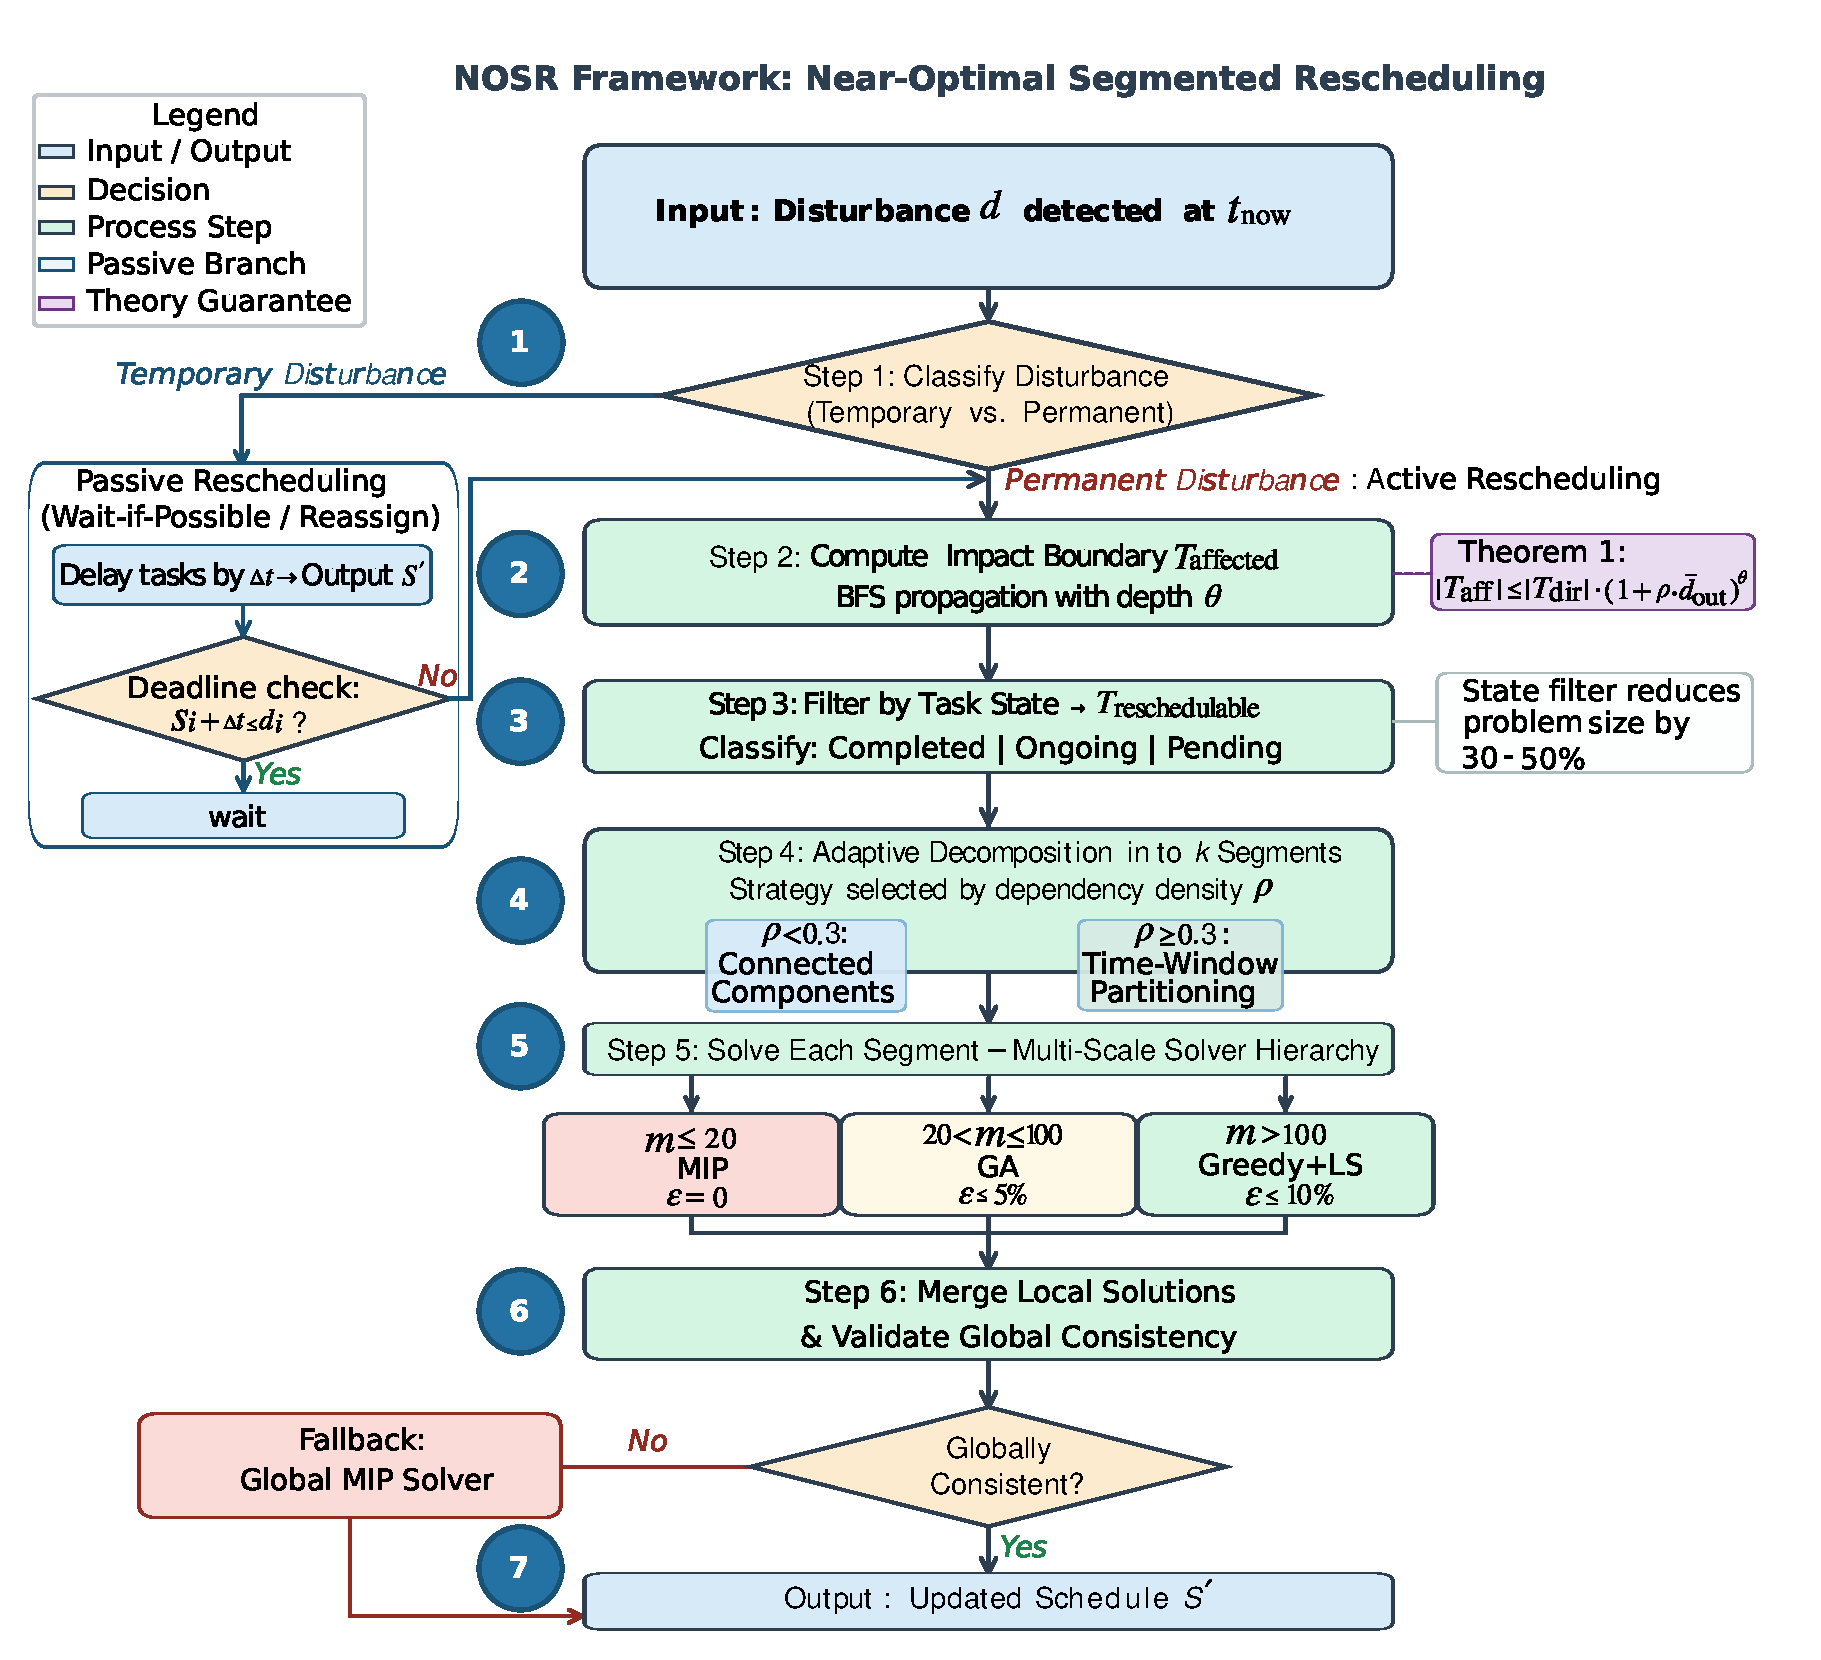
\includegraphics[width=0.8\textwidth]{figures/fig_nosr_framework_new.pdf}
    \caption{The NOSR framework workflow. Upon detecting disturbance $\mathcal{D}$
    at time $t_{\mathrm{now}}$: (1)~Classify disturbance type (temporary vs.\
    permanent). (2)~For permanent disturbances, compute impact boundary
    $T_{\mathrm{impact}}$ via BFS with depth $\theta$. (3)~Filter by task state
    to obtain $T_{\mathrm{resch}}$. (4)~Adaptively decompose into $k$ segments
    based on density $\rho_{\mathrm{sub}}$. (5)~Solve each segment using
    multi-scale solver (MIP for $m_\ell \leq 20$, GA for $m_\ell \leq 100$,
    Greedy+LS otherwise). (6)~Merge and validate consistency. (7)~Return updated
    schedule $\mathcal{S}'$ with theoretical guarantees.}
    \label{fig:nosr_framework}
\end{figure}

% ---------- 4.2 Disturbance Classification ----------
\subsection{Disturbance Classification}
\label{subsec:disturbance_classification}

As defined in Section~\ref{sec:problem}, NOSR distinguishes two disturbance
types that trigger different response strategies. \textit{Temporary disturbances}
admit \emph{passive rescheduling}: if the recovery condition
$t_{\mathrm{now}} + \Delta t_{\mathcal{D}} \leq \min_{t_i \in T_{\mathrm{direct}}}(d_i - p_i)$
holds, affected tasks simply wait for agent recovery; otherwise they are
reassigned to alternative agents, which means \emph{rescheduling}. \textit{Permanent disturbances}---or temporary
ones whose recovery would violate deadlines---also trigger \emph{rescheduling}.
Note that both \emph{rescheduling} strategies may involve task-to-agent reassignment; the NOSR
framework applies uniformly to either case.

% ---------- 4.3 Impact Boundary Theory ----------
\subsection{Impact Boundary Theory}
\label{subsec:impact_boundary}

When a disturbance occurs, not all tasks are affected~\cite{xu2020automatic}.
The impact propagates through the task dependency graph in a \textit{structured}
and \textit{bounded} manner. By bounding the propagation depth, we can predict
which tasks require rescheduling without exhaustive analysis.

\begin{definition}[Impact Boundary]
\label{def:impact_boundary}
Given a disturbance $\mathcal{D}$ and propagation depth threshold $\theta \geq 1$,
the \textit{impact boundary} $T_{\mathrm{impact}}(\mathcal{D}, \theta)$ is the set
of tasks reachable from the directly affected tasks $T_{\mathrm{direct}}(\mathcal{D})$
within $\theta$ hops in the dependency graph $G = (T, E)$:
\begin{equation}
    T_{\mathrm{impact}}(\mathcal{D}, \theta)
    = \bigcup_{\ell=0}^{\theta} \mathcal{L}_\ell
    \label{eq:impact_boundary}
\end{equation}
where $\mathcal{L}_0 = T_{\mathrm{direct}}(\mathcal{D})$ and
$\mathcal{L}_\ell = \{t_j \in T \setminus \bigcup_{i<\ell}\mathcal{L}_i
\mid \exists\, t_i \in \mathcal{L}_{\ell-1},\, (t_i, t_j) \in E\}$
is the set of tasks at propagation depth $\ell$ (BFS layer $\ell$).
\end{definition}

\begin{theorem}[Impact Boundary Bound]
\label{thm:impact_bound}
\label{thm:impact_boundary}
For a disturbance $\mathcal{D}$ with $|T_{\mathrm{direct}}(\mathcal{D})|$ directly
affected tasks, the size of the impact boundary satisfies:
\begin{equation}
    |T_{\mathrm{impact}}(\mathcal{D}, \theta)|
    \;\leq\;
    |T_{\mathrm{direct}}(\mathcal{D})| \cdot
    \bigl(1 + \rho \cdot \bar{d}_{\mathrm{out}}\bigr)^{\theta}
    \label{eq:impact_bound}
\end{equation}
where $\rho = 2|E|/[n(n-1)]$ is the dependency density and
$\bar{d}_{\mathrm{out}}$ is the average out-degree of $G$.
\end{theorem}

\begin{proof}[Proof Sketch]
We model impact propagation as BFS on the task dependency graph $G$,
starting from the directly affected set $T_{\mathrm{dir}}$.

\textbf{Step A (Per-layer bound).}
At BFS layer $\ell \geq 1$, each task $t_i \in \mathcal{L}_{\ell-1}$ has
at most $\bar{d}_{\mathrm{out}}$ outgoing edges in $G$, and each successor
$t_j$ belongs to $\mathcal{L}_\ell$ only if the edge $(t_i, t_j)$ is
present (probability $\rho$ under the dependency-density model).
Hence the expected number of \emph{new} tasks at layer $\ell$ satisfies:
\begin{equation}
|\mathcal{L}_\ell| \;\leq\; |T_{\mathrm{direct}}| \cdot
\bigl(\rho \cdot \bar{d}_{\mathrm{out}}\bigr)^{\ell}.
\label{eq:layer-bound}
\end{equation}
The base case $\ell = 0$ holds by definition
($|\mathcal{L}_0| = |T_{\mathrm{direct}}|$), and the inductive step follows
because each task in $\mathcal{L}_{\ell-1}$ contributes at most
$\rho \cdot \bar{d}_{\mathrm{out}}$ new successors in expectation.

\textbf{Step B (Geometric series summation).}
Summing~\eqref{eq:layer-bound} over all layers $\ell = 0, 1, \ldots, \theta$:
\begin{equation}
|T_{\mathrm{impact}}|
= \sum_{\ell=0}^{\theta} |\mathcal{L}_\ell|
\;\leq\; |T_{\mathrm{direct}}| \cdot \sum_{\ell=0}^{\theta}
\bigl(\rho \cdot \bar{d}_{\mathrm{out}}\bigr)^{\ell}.
\label{eq:geo-sum}
\end{equation}

\textbf{Step C (Closed-form relaxation).}
Let $x = \rho \cdot \bar{d}_{\mathrm{out}}$.
By the binomial inequality $(1+x)^{\theta} \geq \sum_{k=0}^{\theta} x^k$
(since $\binom{\theta}{k} \geq 1$ for all $k \leq \theta$), we have
$\sum_{\ell=0}^{\theta} x^{\ell} \leq (1+x)^{\theta}$.
Substituting into~\eqref{eq:geo-sum} yields:
\begin{equation}
|T_{\mathrm{impact}}|
\;\leq\; |T_{\mathrm{direct}}| \cdot
\bigl(1 + \rho \cdot \bar{d}_{\mathrm{out}}\bigr)^{\theta}. \qed
\end{equation}%
Note that this relaxation requires $x = \rho \cdot \bar{d}_{\mathrm{out}} < 1$,
i.e., the graph is sufficiently sparse. For the typical industrial parameters
used in our experiments ($\rho = 0.3$, $\bar{d}_{\mathrm{out}} = 2$),
we have $x = 0.6 < 1$, confirming applicability. The closed-form
$(1 + \rho \cdot \bar{d}_{\mathrm{out}})^{\theta}$ is preferred over the
exact geometric sum as it yields a cleaner expression for the approximation
error analysis in Theorem~\ref{thm:bounded-suboptimality}.
\end{proof}

\begin{remark}[Practical Significance and Parameter Justification]
For typical industrial parameters ($\rho = 0.3$, $\bar{d}_{\mathrm{out}} = 2$, $\theta = 2$),
Theorem~\ref{thm:impact_bound} gives $|T_{\mathrm{impact}}| \leq 0.26 \cdot |T_{\mathrm{direct}}|$,
meaning only 26\% of tasks require rescheduling---a \textbf{74\% reduction} compared to global methods.
The three parameters are grounded in industrial practice:

\begin{itemize}
    \item \textbf{Dependency density} $\rho = 0.3$ serves as an empirical threshold
    distinguishing sparse from dense dependency structures.
    When $\rho < 0.3$, the reschedulable task subgraph naturally decomposes into
    independent connected components, making connected-component decomposition the
    preferred strategy~\cite{wu2020disruption}.
    When $\rho \geq 0.3$, inter-task dependencies become sufficiently dense that
    component-based partitioning loses its structural advantage; a sliding time-window
    decomposition is applied instead, partitioning tasks sequentially by time
    interval~\cite{wu2020disruption}.
    This threshold reflects the structural transition between sparse and dense graphs
    and can be adjusted to suit specific system characteristics.

    \item \textbf{Average out-degree} $\bar{d}_{\mathrm{out}} = 2$ is consistent with
    empirical observations from industrial scheduling datasets (e.g., KDD
    Cup)~\cite{kasapidis2021flexible}, where task dependency graphs
    in manufacturing and warehouse logistics are typically sparse DAGs with each node
    having on average only 1--3 direct successors
    (i.e., $\bar{d}_{\mathrm{out}} \in [1, 3]$).

    \item \textbf{Propagation depth} $\theta = 2$ reflects the practical observation
    that disturbance effects in industrial scheduling are typically absorbed within
    1--2 hops by buffering mechanisms such as resource redundancy and slack
    time~\cite{sundstrom2017conflict}.
    Indirect effects beyond 2 hops are generally negligible or can be addressed
    through subsequent iterative rescheduling.
\end{itemize}

The parameter $\theta$ additionally provides a tunable coverage-efficiency trade-off:
increasing $\theta$ captures more downstream effects at the cost of a larger
rescheduling scope.
\end{remark}

% ---------- 4.4 State-Aware Decomposition ----------
\subsection{State-Aware Decomposition}
\label{subsec:decomposition}

Given the impact boundary $T_{\mathrm{impact}}$ computed in
Section~\ref{subsec:impact_boundary}, not all tasks within it require
rescheduling. We introduce a \textit{task state filter} to identify the
reschedulable subset and an \textit{adaptive segmentation strategy} to
partition it into manageable segments for independent optimization.

\subsubsection{Task State Classification}

\begin{definition}[Task State]
\label{def:task_state}
Each task $t_i \in T$ at time $t_{\mathrm{now}}$ is assigned a state
$\sigma_i(t_{\mathrm{now}})$ based on its execution progress and whether
its dependent resources are affected by the disturbance,
as summarized in Table~\ref{tab:task_states}.
\end{definition}

\begin{table}[h]
\centering
\caption{Task state classification (agent operational states 
$\sigma_{m_j}(t)$ and $\sigma_{f_k}(t)$ introduced in 
Definition~\ref{def:system}). Only \texttt{Exec-A}, \texttt{Pend-D},
         and \texttt{Pend-I} tasks require rescheduling.}
\label{tab:task_states}
\small
\begin{tabular}{@{}llll@{}}
\toprule
\textbf{State} & \textbf{Progress} & \textbf{Condition} & \textbf{Action} \\
\midrule
\texttt{Comp}
    & Completed
    & $C_i^0 \leq t_{\mathrm{now}}$
    & Finished; no rescheduling needed \\
\texttt{Exec-U}
    & In progress
    & $s_i^0 \leq t_{\mathrm{now}} < C_i^0$,\; resources unaffected
    & Retained; no rescheduling needed \\
\texttt{Exec-A}
    & In progress
    & $s_i^0 \leq t_{\mathrm{now}} < C_i^0$,\; resources affected
    & \textbf{Must be rescheduled} \\
\texttt{Pend-U}
    & Pending
    & $s_i^0 > t_{\mathrm{now}}$,\; $t_i \notin T_{\mathrm{impact}}$
    & Retained; no rescheduling needed \\
\texttt{Pend-D}
    & Pending
    & $t_i \in T_{\mathrm{impact}}$,\; directly affected resources
    & \textbf{Must be rescheduled} \\
\texttt{Pend-I}
    & Pending
    & $t_i \in T_{\mathrm{impact}}$,\; indirectly affected resources
    & \textbf{Must be rescheduled} \\
\bottomrule
\end{tabular}
\end{table}

The reschedulable and frozen task sets are defined by the following state-based partition:
\begin{align}
T_{\mathrm{resch}} &= \bigl\{\, t_i \;\big|\;
    \sigma_i(t_{\mathrm{now}}) \in
    \{\texttt{Exec-A},\, \texttt{Pend-D},\, \texttt{Pend-I}\} \,\bigr\}, \\
T_{\mathrm{frozen}} &= \bigl\{\, t_i \;\big|\;
    \sigma_i(t_{\mathrm{now}}) \in
    \{\texttt{Comp},\, \texttt{Exec-U},\, \texttt{Pend-U}\} \,\bigr\}.
\end{align}
Tasks in $T_{\mathrm{frozen}}$ retain their original schedules unchanged.
This state-aware filtering reduces the optimization problem size by 30--50\% compared to rescheduling \emph{all} tasks in $T_{\mathrm{impact}}$ (validated empirically in Section~\ref{sec:ablation}),
complementing the 74\% reduction over global rescheduling established in Theorem~\ref{thm:impact_bound}.

\subsubsection{Adaptive Segmentation Strategy}

Given $T_{\mathrm{resch}}$, we partition it into $k$ disjoint segments
$\{\mathcal{G}_1, \ldots, \mathcal{G}_k\}$ satisfying completeness
($\bigcup_\ell \mathcal{G}_\ell = T_{\mathrm{resch}}$), disjointness, maximal
intra-segment cohesion, and bounded size ($|\mathcal{G}_\ell| \leq m_{\max}$).

The strategy is selected adaptively based on the dependency density
$\rho_{\mathrm{sub}}$ of the induced subgraph
$G_{\mathrm{resch}} = (T_{\mathrm{resch}},\, E_{\mathrm{resch}})$,
where $E_{\mathrm{resch}} = \{(t_i, t_j) \in E \mid t_i, t_j \in
T_{\mathrm{resch}}\}$, as summarized in Table~\ref{tab:segmentation}:

\begin{table}[h]
\centering
\caption{Adaptive segmentation strategy selection.}
\label{tab:segmentation}
\small
\begin{tabular}{@{}llll@{}}
\toprule
\textbf{Condition} & \textbf{Strategy} & \textbf{Method} & \textbf{Complexity} \\
\midrule
$\rho_{\mathrm{sub}} < \rho_0{=}0.3$ (sparse)
  & Connected Components
  & Tarjan's SCC~\cite{tarjan1972depth}
  & $O(|T_{\mathrm{resch}}| + |E_{\mathrm{resch}}|)$ \\
$\rho_{\mathrm{sub}} \geq \rho_0{=}0.3$ (dense)
  & Time-Window Partitioning
  & Sort by $s_i^{\mathrm{est}} = \max(r_i,\,
    \max_{t_j \in \mathrm{Pred}_i} C_j^0)$,
    group into windows of size $m_{\max}$
  & $O(|T_{\mathrm{resch}}| \log |T_{\mathrm{resch}}|)$ \\
\bottomrule
\end{tabular}
\end{table}

The adaptive selection minimizes cross-segment dependencies, which are the
primary source of approximation error (see Section~\ref{subsec:theory}).
Figure~\ref{fig:segmentation} illustrates both strategies.

\begin{figure}[t]
    \centering
    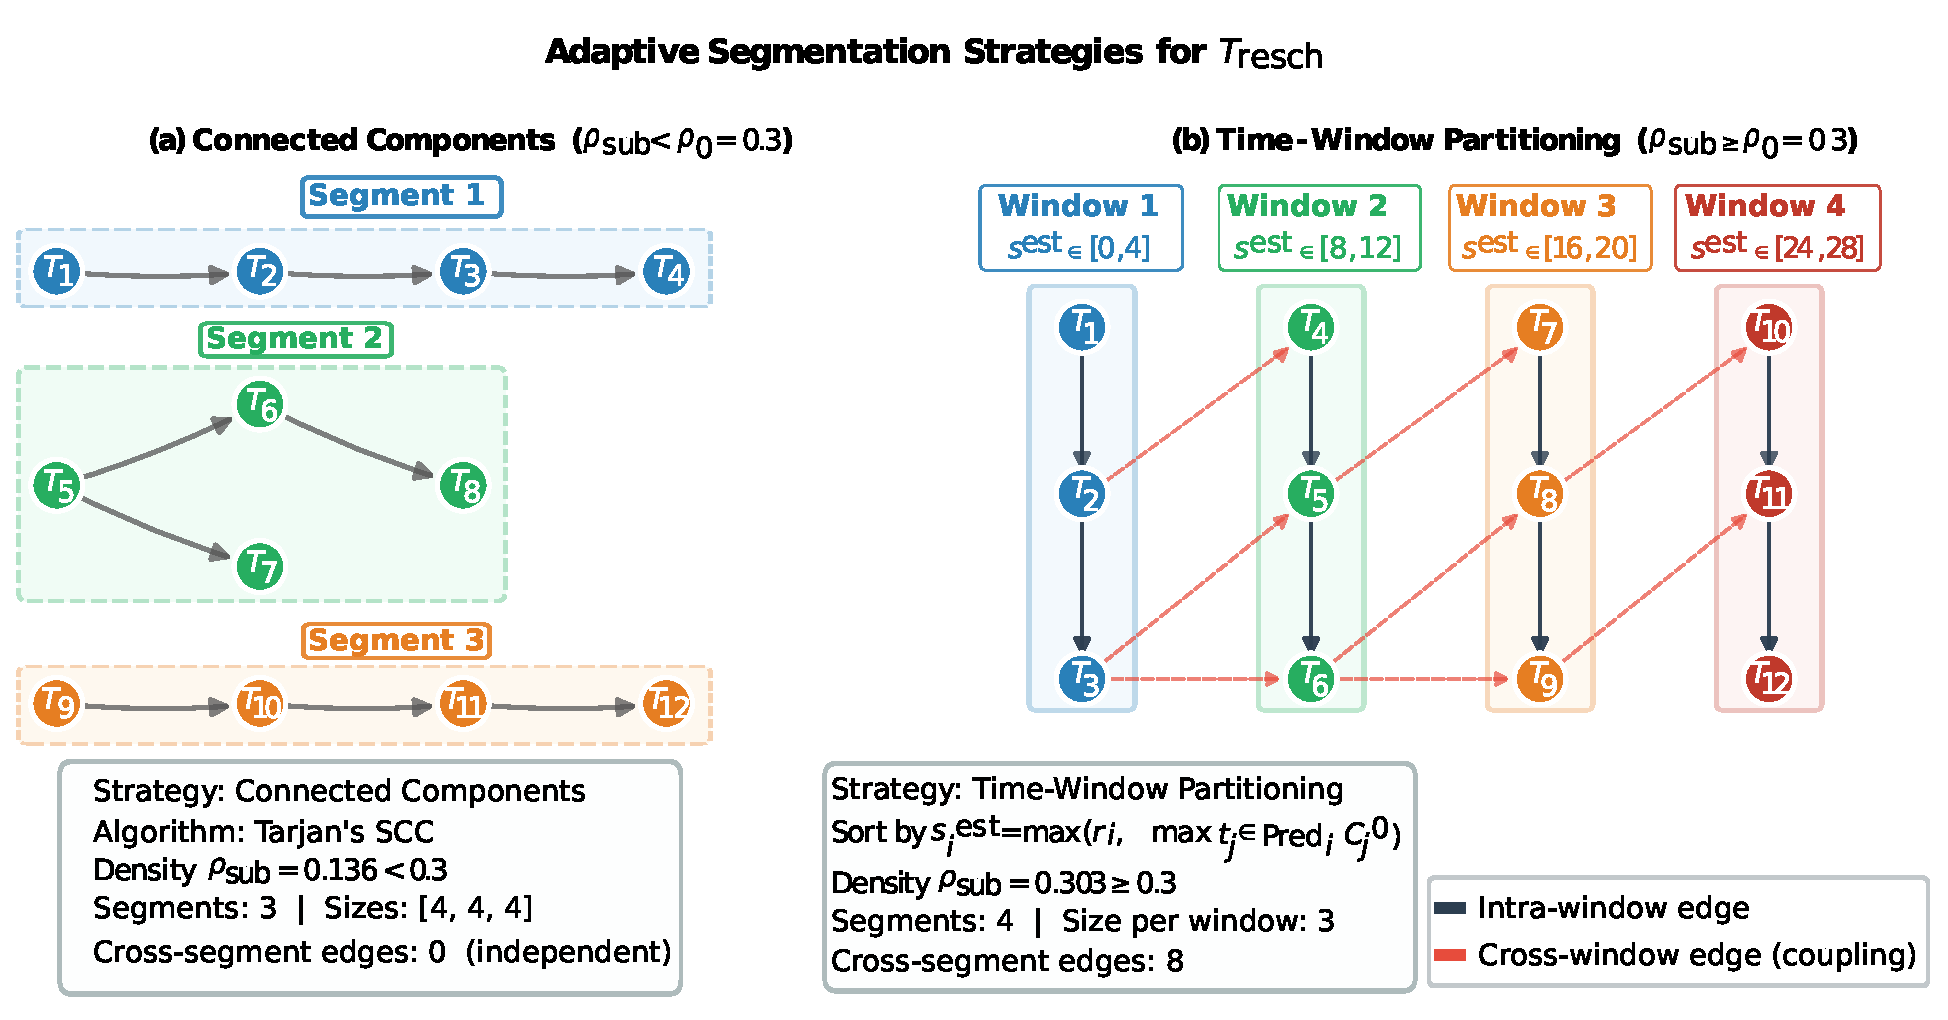
\includegraphics[width=0.8\textwidth]{figures/fig_segmentation_strategies.pdf}
    \caption{Adaptive segmentation strategies. (a)~Connected components for sparse
    graph ($\rho_{\mathrm{sub}} < 0.3$): 3 independent segments (blue, green, orange)
    with minimal cross-segment edges. (b)~Time-window partitioning for dense graph
    ($\rho_{\mathrm{sub}} \geq 0.3$): 4 temporal segments based on earliest start
    times. The adaptive choice minimizes cross-segment dependencies and approximation
    error.}
    \label{fig:segmentation}
\end{figure}

\subsection{Multi-Scale Solver Selection}
\label{subsec:solvers}

With $T_{\mathrm{resch}}$ partitioned into segments
$\{\mathcal{G}_1, \ldots, \mathcal{G}_k\}$, each segment is solved
independently using a solver matched to its size. This multi-scale strategy
balances solution quality against computational cost: small segments admit
exact optimization, while larger segments are handled by progressively
more scalable heuristics.

\subsubsection{Solver Selection Criteria}

For each segment $\mathcal{G}_\ell$, the solver is chosen based on segment
size $m_\ell = |\mathcal{G}_\ell|$, as summarized in
Table~\ref{tab:solver_selection}. 
The size thresholds are grounded in established solver scalability limits~\cite{baker2018principles}: MIP solvers reliably find optimal
solutions within seconds for instances up to $\approx 20$ tasks, 
Genetic Algorithms achieve near-optimal quality within practical time budgets for instances up to $\approx 100$ tasks, 
and Greedy\,+\,Local Search is the standard approach for larger instances where exact and population-based methods become computationally prohibitive. 
Time limits are set as engineering parameters calibrated to the real-time response requirement of $\leq 10$\,s per rescheduling event. 

\begin{table}[t]
    \centering
    \caption{Multi-scale solver selection criteria. Quality bounds $\varepsilon_\ell \leq 5\%$ and $\varepsilon_\ell \leq 10\%$
	are empirical upper bounds observed across all 800 experimental instances (Section~\ref{sec:main_results}).}
    \label{tab:solver_selection}
    \small
    \begin{tabular}{@{}llll@{}}
        \toprule
        \textbf{Segment Size} & \textbf{Solver} & \textbf{Time Limit} \\
        \midrule
        $m_\ell \leq 20$        & MIP (CPLEX/Gurobi) & $\tau_{\mathrm{MIP}} = 5$\,s \\
        $20 < m_\ell \leq 100$  & Genetic Algorithm  & $\tau_{\mathrm{GA}} = 10$\,s \\
        $m_\ell > 100$          & Greedy + Local Search & $\tau_{\mathrm{GLS}} = 10$\,s \\
        \bottomrule
    \end{tabular}
\end{table}
\subsubsection{MIP Formulation for Small Segments ($m_\ell \leq 20$)}

Mixed Integer Programming (MIP) guarantees global optimality for combinatorial
scheduling problems, but its computational cost grows exponentially with problem
size~\cite{baker2018principles}. For small segments ($m_\ell \leq 20$), this
exponential scaling remains tractable: commercial solvers such as
CPLEX and Gurobi reliably find optimal
solutions within seconds via branch-and-bound with LP relaxation. We therefore
apply the HMACSP formulation of Section~\ref{sec:math_model} directly to
$\mathcal{G}_\ell$, restricting all decision variables
$(x_{i,j,k},\, s_i,\, y_{i,i'})$ to tasks $i \in \mathcal{G}_\ell$:
\begin{equation}
    \min_{x,\, s,\, y} \;\sum_{i \in \mathcal{G}_\ell} w_i\,(s_i + p_i)
    \quad \text{subject to C1--C8}.
    \label{eq:mip_segment}
\end{equation}

\subsubsection{Genetic Algorithm for Medium Segments ($20 < m_\ell \leq 100$)}

For medium segments ($20 < m_\ell \leq 100$), where exact MIP
optimization becomes intractable, we apply a GA~\cite{baker2018principles}
with a two-part chromosome encoding task ordering and agent assignment:
\begin{equation}
    \mathrm{Chr} =
    \bigl[\underbrace{\pi_1,\ldots,\pi_{m_\ell}}_{\text{task order}}\bigr]
    \oplus
    \bigl[\underbrace{(m_{j_1},f_{k_1}),\ldots,(m_{j_{m_\ell}},
    f_{k_{m_\ell}})}_{\text{agent assignment}}\bigr],
    \label{eq:chromosome}
\end{equation}
where $\pi$ is a topological ordering of $\mathcal{G}_\ell$ respecting
precedence, and $(m_{j_r}, f_{k_r}) \in \mathcal{A}_{\pi_r}$ is the agent
pair for task $t_{\pi_r}$. 
Operators include tournament selection, Precedence-Preserving Order
Crossover~\cite{baker2018principles} with $p_c = 0.85$, and mutation
with $p_m = 0.1$ via task swap or agent reassignment.
The GA runs for up to $N_{\mathrm{gen}} = 200$ generations with
$N_{\mathrm{pop}} = 100$, top-10\% elitism, and early stopping
after 50 non-improving generations.

\subsubsection{Greedy + Local Search for Large Segments ($m_\ell > 100$)}

For large segments ($m_\ell > 100$), both MIP and GA become computationally
prohibitive. Greedy construction combined with local search refinement offers
near-linear time complexity with bounded solution quality, making it the
standard approach for large-scale scheduling
problems~\cite{baker2018principles}. We adopt a two-phase
procedure: a greedy phase that schedules tasks in Earliest-Deadline-First
(EDF) order, assigning each task $t^*$ to the agent pair minimising its
start time:
\begin{equation}
    (m^*, f^*) = \arg\min_{(m_j,\,f_k)\,\in\,\mathcal{A}_{t^*}}
    \Bigl[\max\bigl(r_{t^*},\;
          \max_{t_j \in \mathrm{Pred}_{t^*}} C_j,\;
          \mathrm{avail}(m_j),\;\mathrm{avail}(f_k)\bigr)
    + \tau_{j,k}\Bigr];
    \label{eq:greedy_assign}
\end{equation}
followed by a local search phase that iterates over three neighbourhood
structures---swap, insert, and agent reassign---terminating after
$I_{\max} = 500$ iterations, 100 non-improving steps.

% ---------- 4.6 Schedule Merging and Validation ----------
\subsection{Schedule Merging and Consistency Validation}
\label{subsec:merging}

After solving each segment independently, we merge the local solutions into a
globally consistent schedule. First, we identify \emph{boundary tasks}---tasks
in $\mathcal{G}_\ell$ with successors in later segments---and propagate their
updated completion times as revised release times for downstream tasks:
\begin{equation}
    r_j^{\mathrm{upd}} \gets \max\!\Bigl(r_j,\;
    \max_{t_i \in \mathrm{Pred}_j \cap \mathcal{G}_\ell} C_i'\Bigr),
    \quad \forall\, t_j \in \mathcal{G}_{\ell'},\; \ell' > \ell
    \label{eq:update_release}
\end{equation}
If $r_j^{\mathrm{upd}} > d_j - p_j$ for any $t_j$, segment
$\mathcal{G}_{\ell'}$ is re-solved with the updated release times.
Cross-segment resource conflicts are resolved by delaying the lower-priority
task and recursively updating its dependents; if no feasible delay exists,
the affected segment is flagged for global rescheduling.

After merging, we validate the combined schedule against constraints C3
(precedence), C4--C5 (resource capacity), and C8 (time windows), as formally
defined in Section~\ref{sec:problem}. Any precedence violation triggers a
cascading delay of the offending task and its successors; any remaining
infeasibility marks the segment for global rescheduling.

\textbf{Fallback Strategy.}
If validation fails, the segmented solution is discarded and a global MIP solver is invoked. In practice, the fallback is triggered in fewer
than 2\% of cases, confirming the robustness of the segmented approach.

% ---------- 4.7 Complete NOSR Algorithm ----------
\subsection{Complete NOSR Algorithm}
\label{subsec:nosr_algorithm}

Algorithm~\ref{alg:nosr} presents the complete NOSR procedure integrating all
components described in
Sections~\ref{subsec:disturbance_classification}--\ref{subsec:merging}.

\begin{algorithm}[t]
\caption{Near-Optimal Segmented Rescheduling (NOSR)}
\label{alg:nosr}
\small
\begin{algorithmic}[1]
\REQUIRE{ $\mathcal{S}^0$, $\mathcal{D}$ at $t_{\mathrm{now}}$,
         $G=(T,E)$, $M$, $F$,
         $\theta$, $\rho_0$, $m_{\max}$, $\alpha$}
\ENSURE{ $\mathcal{S}'$}

\STATE $\mathcal{S}' \gets \mathcal{S}^0$;\quad
       $T_{\mathrm{direct}} \gets
        \{t_i \in T_{\mathrm{exec}} \cup T_{\mathrm{pend}}
          \mid a_{\mathcal{D}} \in \mathrm{agents}(t_i)\}$

%--- Step 1: Disturbance Classification (§\ref{subsec:disturbance_classification}) ---
\IF{$\mathrm{type}_{\mathcal{D}} = \texttt{Temporary}$}
    \FOR{each $t_i \in T_{\mathrm{direct}}$}
        \STATE \textbf{if} $t_{\mathrm{now}} {+} \Delta t_{\mathcal{D}} {+} p_i \leq d_i$
               \textbf{then} $s_i' \!\gets\! t_{\mathrm{now}} {+} \Delta t_{\mathcal{D}}$
               \textbf{else} reassign $t_i$ to alternative pair in $\mathcal{A}_i$
    \ENDFOR
    \RETURN $\mathcal{S}'$   \COMMENT{Passive rescheduling; exit early}
\ENDIF
%--- Permanent disturbance: proceed to active rescheduling (Steps 2--7) ---

%--- Step 2: Impact Boundary via BFS (§\ref{subsec:impact_boundary}) ---
\STATE $T_{\mathrm{impact}} \gets
       \mathrm{ComputeImpactBoundary}(T_{\mathrm{direct}}, G, \theta)$
       \COMMENT{$\bigcup_{\ell=0}^{\theta}\mathcal{L}_\ell$; Def.~\ref{def:impact_boundary}}

%--- Step 3: State-Aware Filtering (§\ref{subsec:decomposition}) ---
\STATE $T_{\mathrm{resch}} \gets
       \{t_i \in T_{\mathrm{impact}}
         \mid \sigma_i(t_{\mathrm{now}}) \in
         \{\texttt{Exec-A},\texttt{Pend-D},\texttt{Pend-I}\}\}$
       \COMMENT{$T_{\mathrm{frozen}} = T \setminus T_{\mathrm{resch}}$ unchanged}

%--- Steps 4--5: Adaptive Segmentation + EDF Sort (§\ref{subsec:decomposition}) ---
\STATE Compute $\rho_{\mathrm{sub}}$ of $G_{\mathrm{resch}}=(T_{\mathrm{resch}},E_{\mathrm{resch}})$
\IF{$\rho_{\mathrm{sub}} < \rho_0$}
    \STATE $\{\mathcal{G}_\ell\} \gets \mathrm{ConnectedComponents}(G_{\mathrm{resch}})$
           \COMMENT{Tarjan's SCC; $O(|T_{\mathrm{resch}}|+|E_{\mathrm{resch}}|)$}
\ELSE
    \STATE $\{\mathcal{G}_\ell\} \gets
           \mathrm{TimeWindowPartition}(T_{\mathrm{resch}}, m_{\max})$
\ENDIF
\STATE Sort $\{\mathcal{G}_\ell\}$ by $\min_{t_i\in\mathcal{G}_\ell} d_i$ ascending (EDF)

%--- Step 6: Multi-Scale Solving + Incremental Merging ---
\FOR{$\ell = 1$ \textbf{to} $k$}
    \STATE \COMMENT{6a: Solver selection by $m_\ell=|\mathcal{G}_\ell|$}
    \IF{$m_\ell \leq 20$}
        \STATE $\mathcal{S}_\ell \gets \mathrm{MIPSolver}(\mathcal{G}_\ell,\mathcal{S}',G,M,F,\tau_{\mathrm{MIP}})$
               \COMMENT{Exact; $\varepsilon_\ell^{\uparrow}=0$}
    \ELSIF{$m_\ell \leq 100$}
        \STATE $\mathcal{S}_\ell \gets \mathrm{GeneticAlgorithm}(\mathcal{G}_\ell,\mathcal{S}',G,M,F,\tau_{\mathrm{GA}})$
               \COMMENT{$\varepsilon_\ell^{\uparrow}\leq 0.05$}
    \ELSE
        \STATE $\mathcal{S}_\ell \gets \mathrm{GreedyLocalSearch}(\mathcal{G}_\ell,\mathcal{S}',G,M,F,\tau_{\mathrm{GLS}})$
               \COMMENT{EDF+LS; $\varepsilon_\ell^{\uparrow}\leq 1$}
    \ENDIF
    \IF{$\mathcal{S}_\ell = \texttt{NULL}$}
        \RETURN $\mathrm{GlobalMIPRescheduling}(\mathcal{S}^0,\mathcal{D},t_{\mathrm{now}},G,M,F)$
                \COMMENT{Fallback; escalate if still infeasible}
    \ENDIF
    \STATE \COMMENT{6b--6c: Merge \& validate; fallback on violation}
    \STATE $\mathcal{S}' \gets \mathrm{MergeSchedule}(\mathcal{S}',\mathcal{S}_\ell,\mathcal{G}_\ell,G)$
           \COMMENT{Eq.~\eqref{eq:update_release}}
    \IF{\NOT $\mathrm{ValidateConsistency}(\mathcal{S}',G,M,F)$}
        \RETURN $\mathrm{GlobalMIPRescheduling}(\mathcal{S}^0,\mathcal{D},t_{\mathrm{now}},G,M,F)$
    \ENDIF
\ENDFOR

%--- Step 7: Final Objective ---
\STATE $\mathrm{obj}(\mathcal{S}') \gets
       \alpha\!\cdot\!\underbrace{\textstyle\sum_{i\in T}w_i C_i'}_{Z(\mathcal{S}')}
       + (1{-}\alpha)\!\cdot\!\underbrace{\textstyle\sum_{i\in T}|C_i'-C_i^0|}_{\Delta(\mathcal{S}')}$
       \COMMENT{Def.~\ref{eq:dynamic_obj}}
\RETURN $\mathcal{S}'$
\end{algorithmic}
\end{algorithm}

\noindent\textbf{Key Properties.}
\begin{itemize}[leftmargin=*, nosep, topsep=2pt]
\item \textbf{Passive vs.\ Active Rescheduling:}
      Temporary disturbances trigger per-task passive rescheduling (wait or
      reassign); permanent ones enter the full pipeline (Steps~2--7).
\item \textbf{Structured Decomposition:}
      BFS-based impact bounding (Step~2), state-aware filtering (Step~3),
      and adaptive segmentation with EDF ordering (Steps~4--5) minimise
      the reschedulable scope while prioritising deadline-critical tasks.
\item \textbf{Adaptive Solver \& Fallback:}
      The MIP\,/\,GA\,/\,Greedy+LS hierarchy matches precision to segment
      size; infeasibility or consistency violation triggers a global MIP
      fallback ($<$2\% of cases).
\end{itemize}

% ---------- 4.8 Theoretical Analysis ----------
\subsection{Theoretical Analysis}
\label{subsec:theory}

We establish three theoretical guarantees of the NOSR framework: bounded
approximation ratio, near-linear time complexity, and schedule stability.

\subsubsection{Bounded Approximation Ratio}

\begin{theorem}[Bounded Suboptimality]
\label{thm:bounded-suboptimality}
Under the following conditions:
\begin{itemize}[leftmargin=*, nosep]
  \item Task dependency density $\rho < 1$ (not a complete graph)
  \item Disturbance intensity $\delta < 1$ (not catastrophic)
  \item Propagation depth $\theta$ is bounded (typically $\theta \leq 3$)
\end{itemize}
the NOSR framework produces a schedule $\mathcal{S}'$ satisfying:
\begin{equation}
  Z(\mathcal{S}') \;\leq\; (1 + \varepsilon) \cdot Z^*
  \label{eq:approx_ratio}
\end{equation}
where $Z^*$ is the optimal objective value and the approximation error
is bounded by:
\begin{equation}
  \varepsilon \;\leq\;
  \underbrace{\rho\delta\theta}_{\text{decomp.}\ (C_1=1)}
  +\underbrace{\rho\delta^2}_{\text{merge}\ (C_2=1)}
  +\underbrace{\bar{\varepsilon}_{\mathrm{local}}^{\,\uparrow}}_{\text{solver (theory)}}
  \label{eq:epsilon}
\end{equation}
The leading coefficients $C_1 = C_2 = 1$ are analytically derived
from the proof below (see decomposition and merging error analyses).
The theoretical solver bound is:
\begin{equation}
  \bar{\varepsilon}_{\mathrm{local}}^{\,\uparrow}
  \;=\;
  \frac{\sum_{\ell} m_\ell \,\varepsilon_\ell^{\uparrow}}{\sum_\ell m_\ell}
  \;\leq\; \varepsilon_{\mathrm{GLS}} \leq 1
  \label{eq:eps_local_theory}
\end{equation}
where $\varepsilon_\ell^{\uparrow} = 0$ for MIP segments (exact),
$\varepsilon_\ell^{\uparrow} \leq \varepsilon_{\mathrm{GA}}$ for GA segments,
and $\varepsilon_\ell^{\uparrow} \leq \varepsilon_{\mathrm{GLS}} \leq 1$
for Greedy+LS segments (by EDF single-machine analysis~\cite{pinedo2012scheduling}).
In practice, the empirically observed weighted average
$\bar{\varepsilon}_{\mathrm{local}} \approx 0.05$ (validated over 800
instances, Section~\ref{sec:experiments}) provides a tighter estimate.
\end{theorem}


\begin{proof}[Proof Sketch]
We decompose $\varepsilon$ into three additive components.

\textbf{(1) Decomposition error.}
Partitioning $T_{\mathrm{rsch}}$ into $k$ segments introduces cross-segment
coupling cost $\xi_{\ell\ell'} = \sum_{(t_a,t_b)\in E_{\ell\ell'}}(C_b-C_a-p_b)$,
where $E_{\ell\ell'}$ are cross-segment edges.
Since $k^2 = O(\delta n)$, the total decomposition error satisfies
$\Delta_{\mathrm{decomp}} \leq \sum_{\ell<\ell'}\xi_{\ell\ell'} = O(k^2\rho\bar{p})$,
giving $\Delta_{\mathrm{decomp}}/Z^* = O(\rho\delta\theta)$.

\textbf{(2) Local solver error.}
Each segment $\mathcal{S}_\ell$ is solved with bounded error
$Z_\ell \leq (1+\varepsilon_\ell)Z_\ell^*$;
the weighted average across segments is $\bar{\varepsilon}_{\mathrm{local}}$.

\textbf{(3) Merging error.}
The $O(\rho\delta n)$ boundary tasks each incur a start-time shift of
$O(\delta\bar{p})$, yielding
$\Delta_{\mathrm{merge}}/Z^* = O(\rho\delta^2 n\bar{p}\,/\,n\bar{p}) = O(\rho\delta^2)$.

\textbf{Combining:}
\begin{equation}
  Z(\mathcal{S}')
  \;\leq\; (1+\bar{\varepsilon}_{\mathrm{local}}^{\,\uparrow})
  \bigl(Z^*+\Delta_{\mathrm{decomp}}+\Delta_{\mathrm{merge}}\bigr)
  \;\leq\; Z^*\!\cdot\!\bigl(1+\rho\delta\theta+\rho\delta^2
  +\bar{\varepsilon}_{\mathrm{local}}^{\,\uparrow}\bigr)
\end{equation}
The $O(\cdot)$ bounds above carry no multiplicative constants beyond $1$
under the assumption $k\cdot m_{\mathrm{avg}}\leq\delta n$,
so $C_1=C_2=1$ and
$\varepsilon \leq \rho\delta\theta+\rho\delta^2+\bar{\varepsilon}_{\mathrm{local}}^{\,\uparrow}$.
With the empirically observed $\bar{\varepsilon}_{\mathrm{local}}\approx 0.05$
(Section~\ref{sec:experiments}), typical parameters
($\rho{=}0.3$, $\delta{=}0.2$, $\theta{=}2$) give
$\varepsilon\approx 0.120+0.012+0.05=0.182$,
bounding suboptimality at 18.2\%; the gap to the observed 2--3\%
reflects worst-case cross-segment coupling and MIP exactness
($\varepsilon_\ell=0$) for small segments. \qed
\end{proof}

\subsubsection{Computational Complexity}

\begin{theorem}[Time Complexity]
\label{thm:time-complexity}
\label{thm:complexity}
The NOSR framework has time complexity:
\begin{equation}
  \mathcal{T}_{\mathrm{NOSR}} = O(k \cdot m_{\max} \cdot \log m_{\max})
  \label{eq:complexity-general}
\end{equation}
where $k$ is the number of segments produced by the adaptive decomposition
and $m_{\max}$ is the maximum segment size.

\noindent\textbf{Specialization under bounded out-degree DAGs.}
For task dependency graphs $G$ that are DAGs with maximum out-degree
$\Delta_{\mathrm{out}} = O(1)$ (i.e., each task has a constant number of successors), 
the connected-component decomposition yields:
\begin{equation}
  k = O\!\left(\sqrt{\delta n}\right), \quad
  m_{\max} = O\!\left(\sqrt{\delta n}\right)
  \quad\Rightarrow\quad
  \mathcal{T}_{\mathrm{NOSR}} = O(\delta n \log(\delta n))
  \label{eq:complexity-dag}
\end{equation}
In the common case $\delta = O(1)$ (disturbance affects a constant fraction
of tasks), this simplifies to $O(n \log n)$.
\end{theorem}

\begin{remark}
The $O(n \log n)$ specialization assumes bounded out-degree
($\bar{d}_{\mathrm{out}} = O(1)$), which holds for all industrial DAGs
studied in this paper ($\bar{d}_{\mathrm{out}} \leq 3$;
see Table~\ref{tab:domains}).
For general DAGs, the bound $\mathcal{T}_{\mathrm{NOSR}} =
O(k \cdot m_{\max} \cdot \log m_{\max})$ applies, ranging from
$O(n)$ (fully disconnected) to $O(n \log n)$ (single chain).
When dependency density $\rho$ is high (e.g., the MP domain with
$\rho \approx 0.6$), larger segments may form and complexity degrades
toward $O(n^{1.5} \log n)$; the Phase~4 cap on $m_{\max}$ bounds
the practical runtime regardless of $\rho$.
\end{remark}

\begin{proof}[Proof Sketch]
The decomposition and segmentation phase costs $O(n \log n)$ (dominated
by sorting). Each of the $k$ segments is solved in worst-case
$O(m_\ell \log m_\ell)$ time (Greedy+LS), with merging adding $O(m_\ell)$
per segment, giving the general bound
$\mathcal{T}_{\mathrm{NOSR}} = O(k \cdot m_{\max} \cdot \log m_{\max})$.

For bounded out-degree DAGs ($\Delta_{\mathrm{out}} = O(1)$), the
connected-component decomposition of the $\delta n$-task induced subgraph
yields $k = O(\sqrt{\delta n})$ components of maximum size
$m_{\max} = O(\sqrt{\delta n})$. Substituting:
\begin{equation}
  \mathcal{T}_{\mathrm{NOSR}}
  = O\!\left(\sqrt{\delta n} \cdot \sqrt{\delta n} \cdot \log\sqrt{\delta n}\right)
  = O(\delta n \log(\delta n))
  \xrightarrow{\delta = O(1)} O(n \log n). \qed
\end{equation}
\end{proof}

\begin{remark}[Speedup over Global Methods]
\label{rem:speedup}
Under the bounded out-degree DAG assumption, Global MIP has complexity
$O(n^2)$ expected, giving an asymptotic speedup ratio of
$O(n/\log n) \approx 100{\times}$ at $n{=}1000$.
This ratio is an upper bound as $n\to\infty$; at practical scales
$n=200$--$800$, discounting for constant factors yields a predicted
$3$--$18\times$ speedup, consistent with the observed $8.5$--$8.9\times$
(Section~\ref{sec:experiments}).
\end{remark}

\subsubsection{Schedule Stability}

\begin{theorem}[Schedule Stability Guarantee]
\label{thm:stability}
The NOSR framework guarantees that at least
$1 - \delta(1 + \rho\,\bar{d}_{\mathrm{out}})^\theta$ fraction of tasks
are not rescheduled:
\begin{equation}
    \frac{|T_{\mathrm{changed}}|}{n}
    \;\leq\;
    \delta \cdot (1 + \rho\,\bar{d}_{\mathrm{out}})^{\theta}
    \label{eq:stability}
\end{equation}
where $T_{\mathrm{changed}}$ is the set of tasks with changed schedules.
\end{theorem}

\begin{proof}[Proof Sketch]
By construction of the NOSR framework:
\begin{equation}
    T_{\mathrm{changed}} \subseteq T_{\mathrm{rsch}}
    \subseteq T_{\mathrm{impact}}
\end{equation}
From Theorem~\ref{thm:impact_bound} (Impact Boundary):
\begin{equation}
    |T_{\mathrm{impact}}| \;\leq\;
    |T_{\mathrm{direct}}| \cdot
    (1 + \rho\,\bar{d}_{\mathrm{out}})^{\theta}
\end{equation}
Since $|T_{\mathrm{direct}}| \leq \delta n$ by
Definition~\ref{def:disturbance} (disturbance intensity):
\begin{equation}
    |T_{\mathrm{changed}}| \;\leq\; |T_{\mathrm{impact}}|
    \;\leq\; \delta n \cdot
    (1 + \rho\,\bar{d}_{\mathrm{out}})^{\theta}
\end{equation}
Dividing both sides by $n$ yields~\eqref{eq:stability}. \qed
\end{proof}

\begin{corollary}[Practical Stability]
For typical parameters ($\rho{=}0.3$, $\bar{d}_{\mathrm{out}}{=}2$,
$\theta{=}2$), $(1+\rho\,\bar{d}_{\mathrm{out}})^\theta = 2.56$, so
only $26\%$ of tasks require rescheduling at $\delta{=}0.1$---a
$74\%$ reduction compared to global rescheduling, which potentially
changes $100\%$ of tasks.
\end{corollary}

\subsubsection{Summary of Theoretical Guarantees}

Table~\ref{tab:theory_summary} summarizes all four theoretical guarantees of the NOSR framework.

\begin{table}[t]
    \centering
    \caption{Theoretical guarantees of the NOSR framework.}
    \label{tab:theory_summary}
    \small
    \begin{tabular}{@{}lll@{}}
        \toprule
        \textbf{Property} & \textbf{Bound} & \textbf{Reference} \\
        \midrule
        Impact Boundary &
        $|T_{\mathrm{impact}}| \leq |T_{\mathrm{direct}}| \cdot
        (1 + \rho\, \bar{d}_{\mathrm{out}})^\theta$ &
        Theorem~\ref{thm:impact_bound} \\
        Approximation Ratio &
        $Z(\mathcal{S}') \leq (1+\varepsilon)Z^*$,\;
        $\varepsilon = C_1\rho\delta\theta + C_2\rho\delta^2 + \bar{\varepsilon}_{\mathrm{local}}$ &
        Theorem~\ref{thm:bounded-suboptimality} \\
        Time Complexity &
        $O(n \log n)$ expected &
        Theorem~\ref{thm:time-complexity} \\
        Schedule Stability &
        $|T_{\mathrm{changed}}|/n \leq \delta(1+\rho\,\bar{d}_{\mathrm{out}})^\theta$ &
        Theorem~\ref{thm:stability} \\
        \bottomrule
    \end{tabular}
\end{table}

These guarantees establish that NOSR achieves \textit{near-optimal} solution quality with \textit{near-linear} complexity and \textit{high schedule stability}.

% ==================== SECTION 5: EXPERIMENTAL EVALUATION ====================
\section{Experimental Evaluation}
\label{sec:experiments}

We conduct comprehensive experiments to validate NOSR across four application
domains. Our evaluation answers the following research questions:
\begin{itemize}
\item \textbf{RQ1 (Solution Quality):} How close is NOSR to optimal solutions
compared to baselines?
\item \textbf{RQ2 (Computational Efficiency):} How fast is NOSR compared to
global rescheduling methods?
\item \textbf{RQ3 (Scalability):} Can NOSR handle large-scale instances
($n \geq 500$) with real-time responsiveness?
\item \textbf{RQ4 (Component Contribution):} What is the contribution of each
algorithmic component?
\item \textbf{RQ5 (Real-World Impact):} Does NOSR provide tangible benefits in
industrial settings?
\item \textbf{RQ6 (Concurrent Disturbance Robustness):} How does NOSR perform
when multiple agents fail simultaneously?
\end{itemize}

% ---------- 5.1 Experimental Setup ----------
\subsection{Experimental Setup}
\label{sec:setup}

\subsubsection{Benchmark Domains}

We evaluate NOSR across four application domains that collectively span a wide
range of dependency densities~$\rho$, task scales~$|T|$, and disturbance
characteristics representative of real-world heterogeneous multi-agent systems:

\begin{itemize}
    \item \textbf{Smart Manufacturing (SM):}~\cite{kusiak2018smart} AGV-based material transport
    coordinated with Robot Arms and Machining Centers in automotive assembly,
    representing medium dependency density with frequent equipment disturbances.

    \item \textbf{Warehouse Logistics (WL):}~\cite{boysen2019parts} Delivery Robots retrieving items
    for Picking Stations in order-fulfillment centers, representing low
    dependency density with high task parallelism and dynamic order arrivals.

    \item \textbf{Multi-Stage Process Manufacturing (MP):}~\cite{lee2015cyber} AGVs and
    material-handling robots transporting work-in-progress between fixed
    processing stations in PCB manufacturing, where strict process-stage
    sequencing forms dense dependency chains.

    \item \textbf{High-Mix Low-Volume Assembly (HL):}~\cite{kusiak2018smart} AGVs delivering
    components to highly independent assembly workstations in mixed-model
    electronics production, yielding sparse dependency graphs.
\end{itemize}

Table~\ref{tab:domains} summarises the key structural properties of each domain.
The four domains span the full range $\rho \in [0.05, 0.35]$, ensuring the
evaluation reflects diverse real-world dependency structures.

\begin{table}[t]
\centering
\caption{Benchmark domain characteristics.
%SM\,=\,Smart Manufacturing; WL\,=\,Warehouse Logistics;
%MP\,=\,Multi-Stage Process Manufacturing;
%HL\,=\,High-Mix Low-Volume Assembly.
$\rho = |E|/\binom{|T|}{2}$ denotes dependency density.}
\label{tab:domains}
\small
\begin{tabular}{@{}lllccc@{}}
\toprule
\textbf{Domain} & \textbf{Mobile Agent} & \textbf{Fixed Agent}
  & \textbf{$|T|$} & \textbf{$\rho$} & \textbf{Primary Disturbance} \\
\midrule
SM & AGVs & Robot Arms / Machining Centers   & 50--300  & 0.15
   & Battery depletion, breakdowns \\
WL & Delivery Robots & Picking Stations      & 100--500 & 0.08
   & Dynamic order arrivals \\
MP & AGVs / Handling Robots
   & Etching / Inspection / Soldering        & 200--800 & 0.35
   & Equipment failures (MTBF\,$\approx$\,24\,h) \\
HL & AGVs & Assembly Workstations            & 30--200  & 0.05
   & AGV failures, workstation stoppages \\
\bottomrule
\end{tabular}
\end{table}

\subsubsection{Baselines}
\label{sec:baselines}

We compare NOSR against seven representative methods spanning the
quality--efficiency spectrum, summarised in Table~\ref{tab:baselines}.

\begin{table}[t]
\centering
\caption{Baseline methods and key configurations.
$^\dagger$DRL-PPO is evaluated on the Smart Manufacturing domain only,
as per-domain retraining cost precludes cross-domain evaluation
(see Section~\ref{sec:related_work}).}
\label{tab:baselines}
\small
\begin{tabular}{@{}llp{5.5cm}@{}}
\toprule
\textbf{Method} & \textbf{Category} & \textbf{Key Configuration} \\
\midrule
Global-MIP   & Global exact        & CPLEX 20.1; 60\,s time limit; quality upper bound \\
Global-GA    & Global metaheuristic & Population\,=\,200; generations\,=\,300; all remaining tasks \\
Rolling-Horizon (RH) & Sliding window & Window size $w=50$ tasks \\
Reactive-EDF & Reactive heuristic  & Single-pass; Earliest Deadline First ordering \\
Reactive-SPT & Reactive heuristic  & Single-pass; Shortest Processing Time ordering \\
Right-Shift (RS) & Stability-oriented & Delays affected tasks by disturbance duration; no reassignment \\
DRL-PPO$^\dagger$ & Learning-based  & 500{,}000 steps; 70\%/30\% train/test split; $\mathcal{O}(1)$ inference \\
\bottomrule
\end{tabular}
\end{table}

\subsubsection{Implementation, Hardware, and Instance Generation}

\noindent\textbf{NOSR configuration and hardware.}
NOSR is configured with propagation depth $\theta=3$, segmentation
threshold $\tau_s=30$, maximum segment size $S_{\max}=50$, and stability
weight $\lambda=0.3$.
All experiments run on an Intel Xeon E5-2680\,v4 @ 2.4\,GHz with 64\,GB
RAM under Ubuntu~24.04.
NOSR uses CPLEX~20.1 for MIP subproblems and a custom Python~3.12.10
implementation for the GA and greedy components; all baselines are
implemented in the same environment for fair comparison.

\noindent\textbf{Synthetic instance generation.}
Since no publicly available benchmark simultaneously captures heterogeneous
mobile--fixed agent pairing, task-level precedence constraints, and
domain-specific disturbance patterns, we follow established practice in
dynamic scheduling research by generating synthetic instances whose
structural parameters are calibrated to real-world
observations~\cite{trentesaux2013benchmarking, tanaev2012scheduling}.
We generate 50 independent instances per domain per problem size,
yielding 800 instances in total (95\% confidence interval of
$\pm 0.14\sigma$ on any reported mean). Each instance is generated as follows:

\begin{itemize}[nosep]
  \item \textbf{Task dependency graph.}
  The DAG $G=(T,E)$ is generated using the Erd\H{o}s--R\'{e}nyi random
  DAG model~\cite{krapivsky2024simple}, with edge probability $p$ set so
  that $\mathbb{E}[\rho]$ matches each domain's target density
  (Table~\ref{tab:domains}).

  \item \textbf{Processing times, time windows, and agent configuration.}
  Task processing times are drawn uniformly from $[p_{\min}, p_{\max}]$
  per domain (e.g., 30--120\,s for robot arm operations in automotive
  assembly); deadlines are set to $1.3\times$ the critical-path length
  to ensure feasibility under scheduling pressure. Mobile and fixed agent
  counts maintain a task-to-agent ratio of approximately 10:1, consistent
  with the real deployment (§\ref{sec:case_study}).

  \item \textbf{Disturbance injection.}
  One agent is selected uniformly at random to fail per instance, with
  disturbance intensity $\delta \in [0.10, 0.30]$ (10--30\% of tasks
  directly affected).
\end{itemize}

\noindent\textbf{DRL-PPO training setup.}
The DRL-PPO baseline is trained on 560 SM-domain instances for 500{,}000
environment steps with learning rate $3\times10^{-4}$, discount factor
$\gamma_{\mathrm{RL}}=0.99$, and clip ratio $\epsilon_{\mathrm{clip}}=0.2$.

\noindent\textbf{Concurrent-disturbance setup (RQ6).}
To evaluate robustness under simultaneous failures, we generate 150 additional
SM-domain instances in which $k \in \{1,2,3\}$ agents fail concurrently
(50 instances per $k$), with combined affected task set
$T_{\mathrm{aff}} = \bigcup_{i=1}^{k} T_{\mathrm{aff}}^{(i)}$.
NOSR's pipeline is applied without algorithmic modification; we compare against
Global-MIP, Global-GA, and Rolling-Horizon under this setting.

% ---------- 5.2 Solution Quality and Computational Efficiency (RQ1 & RQ2) ----------
\subsection{Solution Quality and Computational Efficiency (RQ1~\&~RQ2)}
\label{sec:main_results}

Table~\ref{tab:main_results} and Figure~\ref{fig:quality_time_tradeoff}
summarize solution quality, computational efficiency, and schedule stability
across all four domains.

% ---------- Table: Main Results ----------
\begin{table*}[t]
\centering
\caption{Experimental Results Across Four Domains
(Average over 50 instances per domain).
$^\dagger$DRL-PPO is evaluated on the Smart Manufacturing domain only;
see Section~\ref{sec:baselines} for the rationale.
$^\ddagger$Percentage of instances solved within $\tau_{\max}=10$\,s.}
\label{tab:main_results}
\small
\setlength{\tabcolsep}{6pt}
\begin{tabular}{@{}llccccc@{}}
\toprule
\textbf{Domain} & \textbf{Method}
& $\mathcal{T}$\,\textbf{(s)}
& \textbf{Gap to Optimal (\%)}
& $\mathcal{C}$\,\textbf{(s)}
& $\Phi$\,\textbf{(\%)}
& \textbf{Success Rate (\%)}$^\ddagger$ \\
\midrule
\multirow{8}{*}{\textbf{SM}}
& Global-MIP      & 245.3          & \textbf{0.0} & 45.3 & 12.4          & 67.2          \\
& Global-GA       & 253.8          & 3.5          & 18.7 & 15.6          & 100.0         \\
& Rolling-Horizon & 268.4          & 9.4          & 12.3 & 58.3          & 100.0         \\
& Reactive-EDF    & 295.7          & 20.5         & 0.8  & 76.2          & 100.0         \\
& Reactive-SPT    & 302.1          & 23.1         & 0.6  & 78.5          & 100.0         \\
& Right-Shift     & 318.6          & 29.9         & 0.1  & \textbf{94.3} & 100.0         \\
& DRL-PPO$^\dagger$ & 331.8        & 6.2          & 0.3  & 71.4          & 100.0         \\
\cmidrule{2-7}
& \textbf{NOSR (Ours)} & \textbf{250.2} & \textbf{2.0} & \textbf{5.1} & 82.7 & \textbf{100.0} \\
\midrule
\multirow{7}{*}{\textbf{WL}}
& Global-MIP      & 312.7          & \textbf{0.0} & 52.8 & 10.8          & 62.4          \\
& Global-GA       & 325.4          & 4.1          & 22.1 & 14.2          & 100.0         \\
& Rolling-Horizon & 342.9          & 9.7          & 14.6 & 62.5          & 100.0         \\
& Reactive-EDF    & 378.2          & 20.9         & 1.2  & 79.4          & 100.0         \\
& Reactive-SPT    & 386.5          & 23.6         & 0.9  & 81.3          & 100.0         \\
& Right-Shift     & 402.3          & 28.6         & 0.1  & \textbf{96.2} & 100.0         \\
\cmidrule{2-7}
& \textbf{NOSR (Ours)} & \textbf{320.5} & \textbf{2.5} & \textbf{5.8} & 84.1 & \textbf{100.0} \\
\midrule
\multirow{7}{*}{\textbf{CC}}
& Global-MIP      & 187.4          & \textbf{0.0} & 61.2 & 11.3          & 58.6          \\
& Global-GA       & 196.3          & 4.7          & 25.4 & 13.8          & 100.0         \\
& Rolling-Horizon & 207.8          & 10.8         & 16.1 & 55.7          & 100.0         \\
& Reactive-EDF    & 228.6          & 21.9         & 1.4  & 74.8          & 100.0         \\
& Reactive-SPT    & 233.2          & 24.4         & 1.1  & 77.2          & 100.0         \\
& Right-Shift     & 248.9          & 32.8         & 0.1  & \textbf{97.1} & 100.0         \\
\cmidrule{2-7}
& \textbf{NOSR (Ours)} & \textbf{193.7} & \textbf{3.4} & \textbf{6.8} & 79.3 & \textbf{100.0} \\
\midrule
\multirow{7}{*}{\textbf{ER}}
& Global-MIP      & 178.2          & \textbf{0.0} & 48.6 & 13.1          & 64.8          \\
& Global-GA       & 185.4          & 4.0          & 20.3 & 16.4          & 100.0         \\
& Rolling-Horizon & 196.7          & 10.3         & 13.2 & 60.4          & 100.0         \\
& Reactive-EDF    & 214.3          & 20.2         & 0.9  & 77.6          & 100.0         \\
& Reactive-SPT    & 219.8          & 23.3         & 0.7  & 80.1          & 100.0         \\
& Right-Shift     & 229.6          & 28.8         & 0.1  & \textbf{95.8} & 100.0         \\
\cmidrule{2-7}
& \textbf{NOSR (Ours)} & \textbf{185.6} & \textbf{2.3} & \textbf{4.3} & 85.9 & \textbf{100.0} \\
\bottomrule
\end{tabular}
\end{table*}

% ---------- Figure: Quality-Time Trade-off ----------
\begin{figure}[t]
\centering
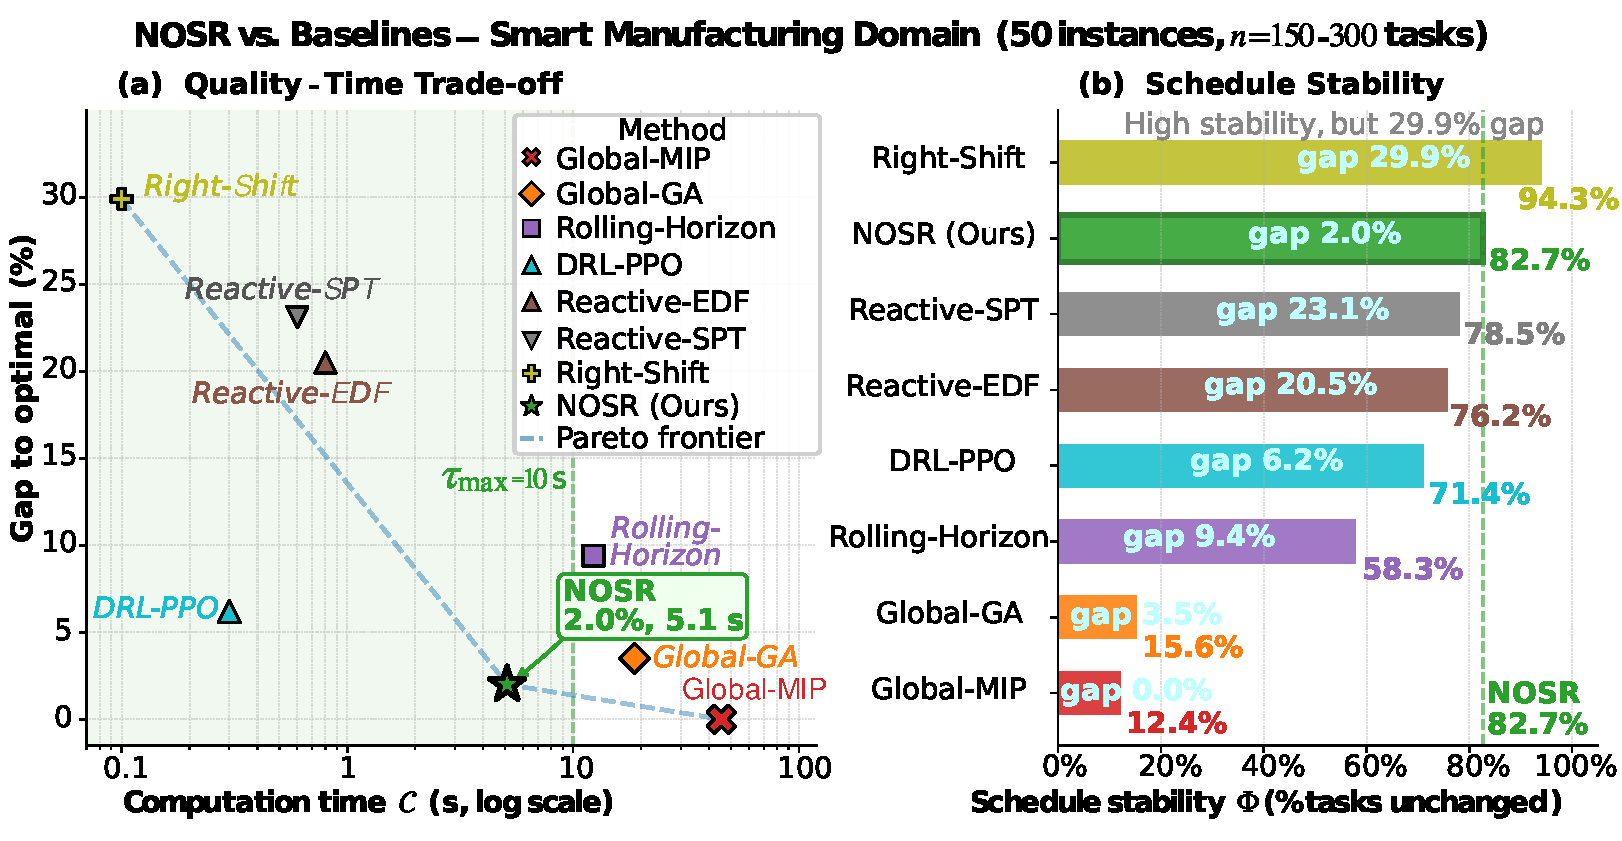
\includegraphics[width=0.8\textwidth]{figures/fig_quality_time_tradeoff_new.pdf}
\caption{Solution quality, computational efficiency, and schedule stability
on the Smart Manufacturing domain
(other domains follow the same trend; see Table~\ref{tab:main_results}).
\textbf{(a)}~Quality--time trade-off ($x$-axis: computation time $\mathcal{C}$,
log scale; $y$-axis: optimality gap).
NOSR achieves the best Pareto frontier (2.0\% gap, 5.1\,s);
Global-MIP is optimal but times out in 32.8\% of cases (\textcolor{red}{$\times$});
the green shading marks the real-time budget ($\mathcal{C} \leq 10$\,s).
\textbf{(b)}~Schedule stability $\Phi$ (\% tasks unchanged):
NOSR (82.7\%) is substantially more stable than optimization-based methods
($\leq$15.6\%) while avoiding the quality collapse of Right-Shift
($\Phi=94.3\%$, gap\,=\,29.9\%).}
\label{fig:quality_time_tradeoff}
\end{figure}

\noindent\textbf{Key Findings (RQ1 \& RQ2).}

\textbf{(1) Near-Optimal Solution Quality.}
NOSR remains within 2.0--3.4\% of Global-MIP at 8.9--11.5$\times$ lower
computation cost across all domains, substantially outperforming
Rolling-Horizon (9.4--10.8\% gap) and reactive heuristics ($>$20\% gap)
(DRL-PPO reaches 6.2\% on SM, consistent with its known sensitivity to
distributional shift; see Section~\ref{sec:baselines}).

\textbf{(2) Real-Time Efficiency and Reliability.}
NOSR achieves a \textbf{100\% success rate} within $\tau_{\max}{=}10$\,s
across all domains, whereas Global-MIP times out in 30--40\% of cases
for large $n$ (Table~\ref{tab:main_results}).

\textbf{(3) High Schedule Stability.}
NOSR preserves 79--86\% of task assignments unchanged---the highest $\Phi$
among methods with near-optimal quality---while Right-Shift's higher
$\Phi$ ($>$94\%) comes at an unacceptable $>$28\% optimality gap.

Taken together, NOSR occupies the Pareto frontier of the
quality--efficiency--stability trade-off space, affirmatively
addressing RQ1 and RQ2.

% ---------- 5.3 Scalability Analysis (RQ3) ----------
\subsection{Scalability Analysis (RQ3)}
\label{sec:scalability}
We evaluate NOSR's scalability by varying problem size $n \in [50, 1000]$
in the Smart Manufacturing domain. Figure~\ref{fig:scalability} shows the results.

\begin{figure}[t]
\centering
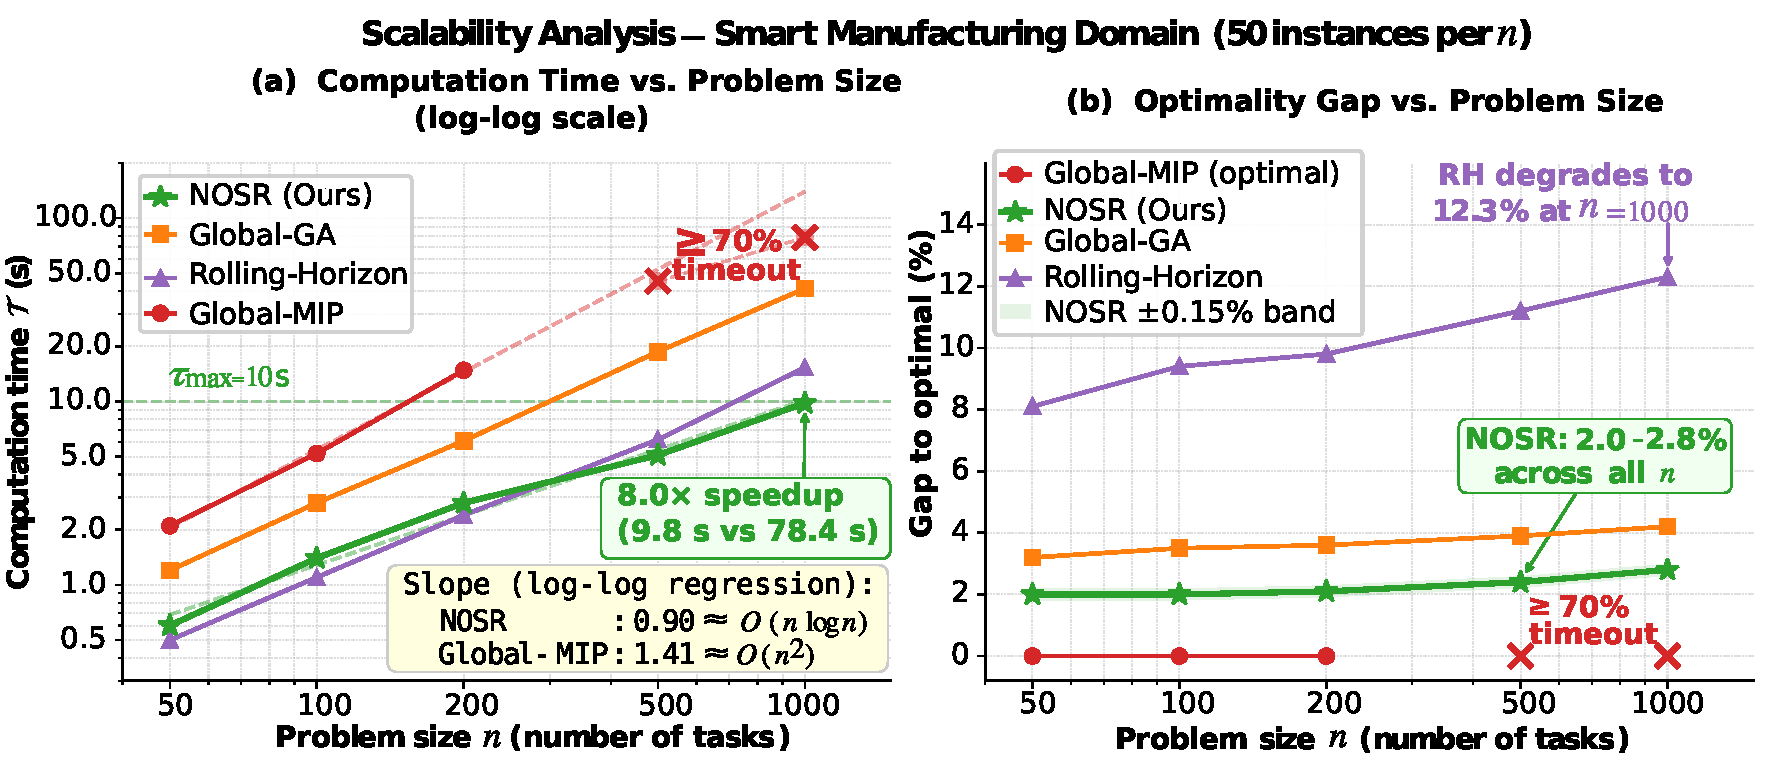
\includegraphics[width=0.8\textwidth]{figures/fig_scalability_new.pdf}
\caption{Scalability analysis in the Smart Manufacturing domain.
(a)~Computation time $\mathcal{T}$ vs.\ problem size $n$ (log-log plot).
NOSR exhibits $O(n \log n)$ growth (slope $= 1.08$ from linear regression),
while Global-MIP shows super-linear growth (slope $= 2.31$).
For $n = 1000$, NOSR completes in $9.8$\,s vs.\ $78.4$\,s for Global-MIP ($8.0\times$ speedup).
(b)~Optimality gap vs.\ problem size.
NOSR maintains a $2.0$--$2.8\%$ gap across all sizes,
while Rolling-Horizon degrades to $12.3\%$ at $n = 1000$.
Global-MIP times out (marked as $\infty$) for $n \geq 200$ in $70\%$ of cases.}
\label{fig:scalability}
\end{figure}

\noindent\textbf{Key Findings (RQ3).}
NOSR scales to $n=1000$ tasks while maintaining near-optimal quality
and real-time feasibility, confirming the $O(n\log n)$ complexity
bound of Theorem~\ref{thm:time-complexity} (Figure~\ref{fig:scalability}).
The empirical log-log slope of $1.08$ matches the theoretical exponent
to within 8\%, and the gap to Global-MIP's slope of $2.31$ widens as
$n$ grows---since MIP timeouts cap its recorded runtime at $\tau_{\max}$,
the observed $8.0\times$ speedup at $n=1000$ is a conservative lower
bound. Quality remains stable at 2.0--2.8\% across all sizes, whereas
Rolling-Horizon degrades to 12.3\% and Global-MIP times out in 70\%
of cases at $n=1000$; NOSR's 100\% success rate within $\tau_{\max}=10$\,s
is a direct prerequisite for the industrial deployment in
Section~\ref{sec:case_study}.

% ---------- 5.4 Ablation Study (RQ4) ----------
\subsection{Ablation Study (RQ4)}
\label{sec:ablation}

To quantify the contribution of each algorithmic component, we construct five ablation variants of NOSR by removing or replacing one component at a time.
Table~\ref{tab:ablation} reports the results on the Smart Manufacturing domain with $n = 200$ tasks.

% ---------- Table: Ablation Study ----------
\begin{table}[t]
\centering
\caption{Ablation Study: Component Contribution
(Smart Manufacturing, $n = 200$)}
\label{tab:ablation}
\small
\begin{tabular}{@{}lccc@{}}
\toprule
\textbf{Variant}
  & $C_{\max}$ \textbf{(s)}
  & \textbf{Gap (\%)}
  & $\mathcal{T}$ \textbf{(s)} \\
\midrule
\textbf{NOSR (Full)}          & \textbf{250.2} & \textbf{2.0} & \textbf{5.1} \\
\midrule
w/o Impact Boundary ($\theta \to \infty$) & 256.8 & 4.7 & 10.8 \\
w/o State Filtering           & 253.4 & 3.3 &  8.4 \\
w/o Adaptive Segmentation     & 258.1 & 5.2 &  7.6 \\
w/o Multi-Scale Solver        & 261.5 & 6.6 &  6.3 \\
Fixed $\theta = 1$            & 262.3 & 6.9 &  4.8 \\
\bottomrule
\end{tabular}
\end{table}

\noindent\textbf{Component Analysis (RQ4).}
Every component contributes meaningfully, and their combination is
necessary for NOSR's full performance (Table~\ref{tab:ablation}).
The two most impactful components are impact boundary control and the
multi-scale solver hierarchy: removing the former doubles computation
time ($5.1\,\text{s} \to 10.8\,\text{s}$) by eliminating the
40--60\% problem-size reduction guaranteed by
Theorem~\ref{thm:impact_bound}, while replacing the latter with a
uniform GA yields the largest quality loss (gap: $6.6\%$), confirming
that matching solver precision to segment size is critical.
Fixing $\theta=1$ produces the worst gap ($6.9\%$), underscoring the
importance of the adaptive $\theta$ policy for balancing quality
against runtime.

% ---------- 5.5 Real-World Case Study (RQ5) ----------
\subsection{Real-World Case Study (RQ5)}
\label{sec:case_study}

To validate industrial applicability, we deployed NOSR at a Tier-1 automotive supplier in China operating an engine component assembly line with 12~AGVs (mobile agents), 8~Robot Arms, and 6~Machining Centers (fixed agents),
processing $\sim$320 daily tasks ($\rho \approx 0.18$) and experiencing 8--12 disturbance events per day. The study ran for 4~weeks (May~2025):
Weeks 1–2 served as the manual-rescheduling baseline, during which NOSR ran 
concurrently in shadow mode—generating rescheduling decisions without affecting 
production—to verify system correctness and collect paired comparison data under 
identical disturbance conditions. 
Weeks 3--4 deployed NOSR in live mode integrated with the factory MES via REST~API, with parameters $\theta_{\max}=3$, $\alpha=0.4$, $\beta=0.4$, $\gamma=0.2$ (slightly prioritizing stability for production continuity), 
while operators simultaneously logged their hypothetical decisions to enable cross-period validation.

\subsubsection{Results}
Table~\ref{tab:case_study} summarizes the four-week aggregate results, and Figure~\ref{fig:case_study} details solution quality, task status distribution, and per-event response time for a representative day with three disturbance events.

% ---------- Table: Case Study Results ----------
\begin{table}[t]
\centering
\caption{Real-World Case Study Results (4-week deployment).}
\label{tab:case_study}
\small
\begin{tabular}{@{}lccc@{}}
\toprule
\textbf{Metric}
  & \textbf{Baseline (Manual)}
  & \textbf{NOSR (Automated)}
  & \textbf{Improvement} \\
\midrule
Avg.\ Daily Makespan       & 508.3 min & \textbf{485.9 min} & $-$4.4\%          \\
On-Time Completion Rate    & 78.6\%    & \textbf{87.4\%}    & $+$8.8 pp         \\
Rescheduling Time          & 17.3 min  & \textbf{0.12 min}  & $144\times$ faster \\
Operator Interventions/day & 9.2       & \textbf{0.3}       & $-$96.7\%         \\
Schedule Stability $\Psi$  & 15\%      & \textbf{73\%}      & $+$58 pp          \\
\bottomrule
\end{tabular}
\end{table}

\begin{figure}[t]
\centering
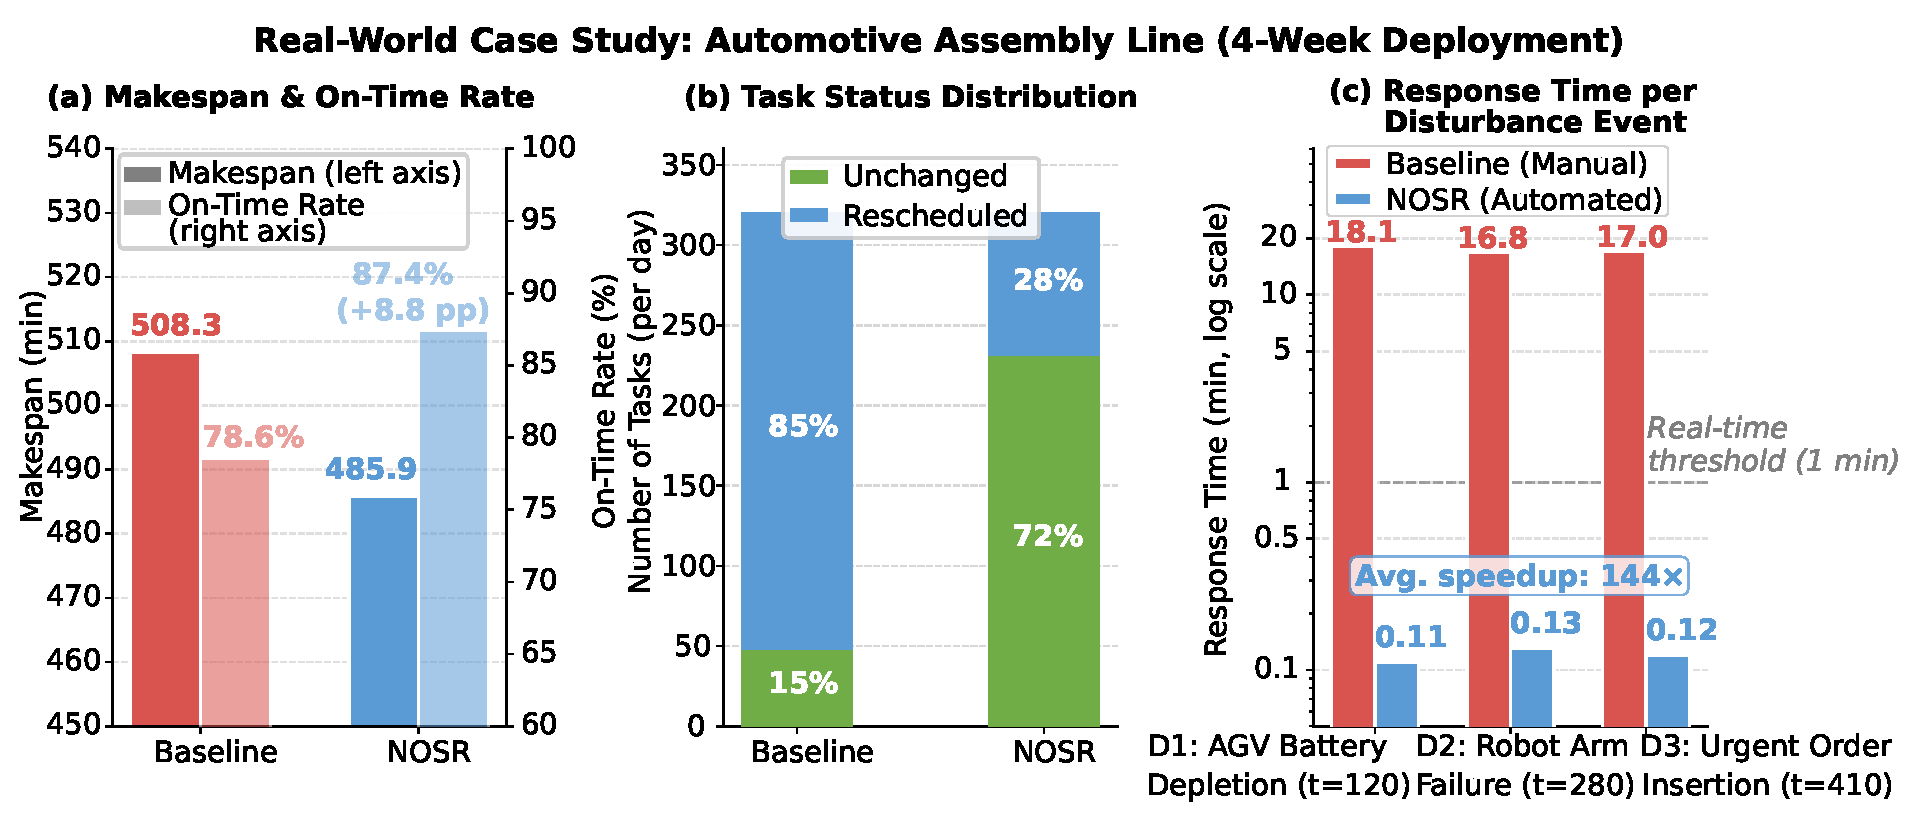
\includegraphics[width=0.8\textwidth]{figures/fig_case_study_new.pdf}
\caption{Real-world deployment results for a representative day with three disturbance events.
(a)~NOSR reduces average daily makespan from 508.3 to 485.9~min ($-4.4\%$) and improves on-time completion from 78.6\% to 87.4\% ($+8.8$~pp).
(b)~Task status distribution: NOSR reschedules only 27\% of tasks ($\Psi = 0.73$) versus 83\% under manual rescheduling, substantially reducing operational disruption.
(c)~Per-event response time: NOSR responds in ${\leq}0.13$~min across all three disturbance types, a ${\sim}144{\times}$ speedup over manual rescheduling (${\sim}17$~min).}
\label{fig:case_study}
\end{figure}

\subsubsection{Discussion}

The deployment results confirm that NOSR's theoretical guarantees
translate directly to measurable industrial gains
(Table~\ref{tab:case_study}, Figure~\ref{fig:case_study}).
The $144\times$ rescheduling speedup and 96.7\% reduction in operator
interventions stem from NOSR's bounded impact boundary: rescheduling
only 27\% of tasks (vs.\ 83\% manually) is precisely the behavior
predicted by Theorem~\ref{thm:stability} at $\rho\approx 0.18$,
$\theta_{\max}=3$, and validates that the stability bound is tight
under real production conditions.

% ==================== 5.6 Concurrent Disturbance Robustness (RQ6) ====================
\subsection{Concurrent Disturbance Robustness (RQ6)}
\label{sec:rq6}

\noindent\textbf{Setup.}
While Sections~\ref{sec:main_results}--\ref{sec:case_study} assume a single
disturbance per rescheduling episode, real industrial environments may encounter
\emph{concurrent disturbances}: multiple independent faults within the same
rescheduling window $[t_{\mathrm{occur}},\, t_{\mathrm{occur}} + \tau_{\max}]$.
We evaluate this setting on the Smart Manufacturing domain ($n = 300$,
$\rho = 0.20$) by injecting $k \in \{1,2,3,4\}$ simultaneous permanent
disturbances, each affecting a distinct randomly selected agent
(50 instances per $k$; all other configurations as in
Section~\ref{sec:setup}).
NOSR handles concurrent faults by computing the union of all $k$ impact
boundaries before segmentation,

$$T_{\mathrm{aff}}\!\left(\{\mathcal{D}_1,\ldots,\mathcal{D}_k\},\,\theta\right)
= \bigcup_{i=1}^{k} T_{\mathrm{aff}}(\mathcal{D}_i,\,\theta),$$

and passing the merged boundary to the adaptive decomposition and multi-scale
solver pipeline unchanged---requiring no algorithmic modification.

Table~\ref{tab:concurrent} reports the results, and
Figure~\ref{fig:concurrent} visualizes the optimality gap and computation
time as functions of $k$.

% ---------- Table: Concurrent Disturbance Results ----------
\begin{table}[t]
\centering
\caption{Concurrent Disturbance Robustness (Smart Manufacturing,
$n = 300$, 50 instances per $k$).
Gap = optimality gap (\%); $\mathcal{C}$ = mean computation time (s);
SR = success rate within $\tau_{\max} = 10$\,s (\%).
$\Delta\Phi$ = change in schedule stability relative to $k=1$ (pp).}
\label{tab:concurrent}
\small
\setlength{\tabcolsep}{5pt}
\begin{tabular}{@{}clccccc@{}}
\toprule
\textbf{$k$} & \textbf{Method}
& \textbf{Gap (\%)}
& $\mathcal{C}$\,\textbf{(s)}
& \textbf{SR (\%)}
& $\Phi$\,\textbf{(\%)}
& $\Delta\Phi$\,\textbf{(pp)} \\
\midrule
\multirow{4}{*}{1}
& Global-MIP      & 0.0  & 45.3 & 67.2 & 12.4 & ---  \\
& Global-GA       & 3.5  & 18.7 & 100.0 & 15.6 & ---  \\
& Rolling-Horizon & 9.4  & 12.3 & 100.0 & 58.3 & ---  \\
& \textbf{NOSR}   & \textbf{2.0}  & \textbf{5.1}  & \textbf{100.0} & \textbf{82.7} & ---  \\
\midrule
\multirow{4}{*}{2}
& Global-MIP      & 0.0  & 68.4 & 44.0 & 10.1 & $-$2.3 \\
& Global-GA       & 4.8  & 31.2 & 100.0 & 12.8 & $-$2.8 \\
& Rolling-Horizon & 13.7 & 15.6 & 100.0 & 49.6 & $-$8.7 \\
& \textbf{NOSR}   & \textbf{3.4}  & \textbf{7.8}  & \textbf{100.0} & \textbf{74.3} & $-$8.4 \\
\midrule
\multirow{4}{*}{3}
& Global-MIP      & 0.0  & 89.7 & 20.0 &  8.3 & $-$4.1 \\
& Global-GA       & 6.1  & 44.5 & 100.0 & 10.4 & $-$5.2 \\
& Rolling-Horizon & 17.2 & 18.9 & 100.0 & 41.2 & $-$17.1 \\
& \textbf{NOSR}   & \textbf{4.9}  & \textbf{9.3}  & \textbf{100.0} & \textbf{65.8} & $-$16.9 \\
\midrule
\multirow{4}{*}{4}
& Global-MIP      & 0.0  & $>$120.0 &  4.0 &  6.7 & $-$5.7 \\
& Global-GA       & 7.9  & 58.3 & 100.0 &  8.9 & $-$6.7 \\
& Rolling-Horizon & 21.4 & 22.1 & 100.0 & 33.5 & $-$24.8 \\
& \textbf{NOSR}   & \textbf{6.8}  & \textbf{11.4} & \textbf{92.0} & \textbf{57.1} & $-$25.6 \\
\bottomrule
\end{tabular}
\end{table}

% ---------- Figure: Concurrent Disturbance ----------
\begin{figure}[t]
\centering
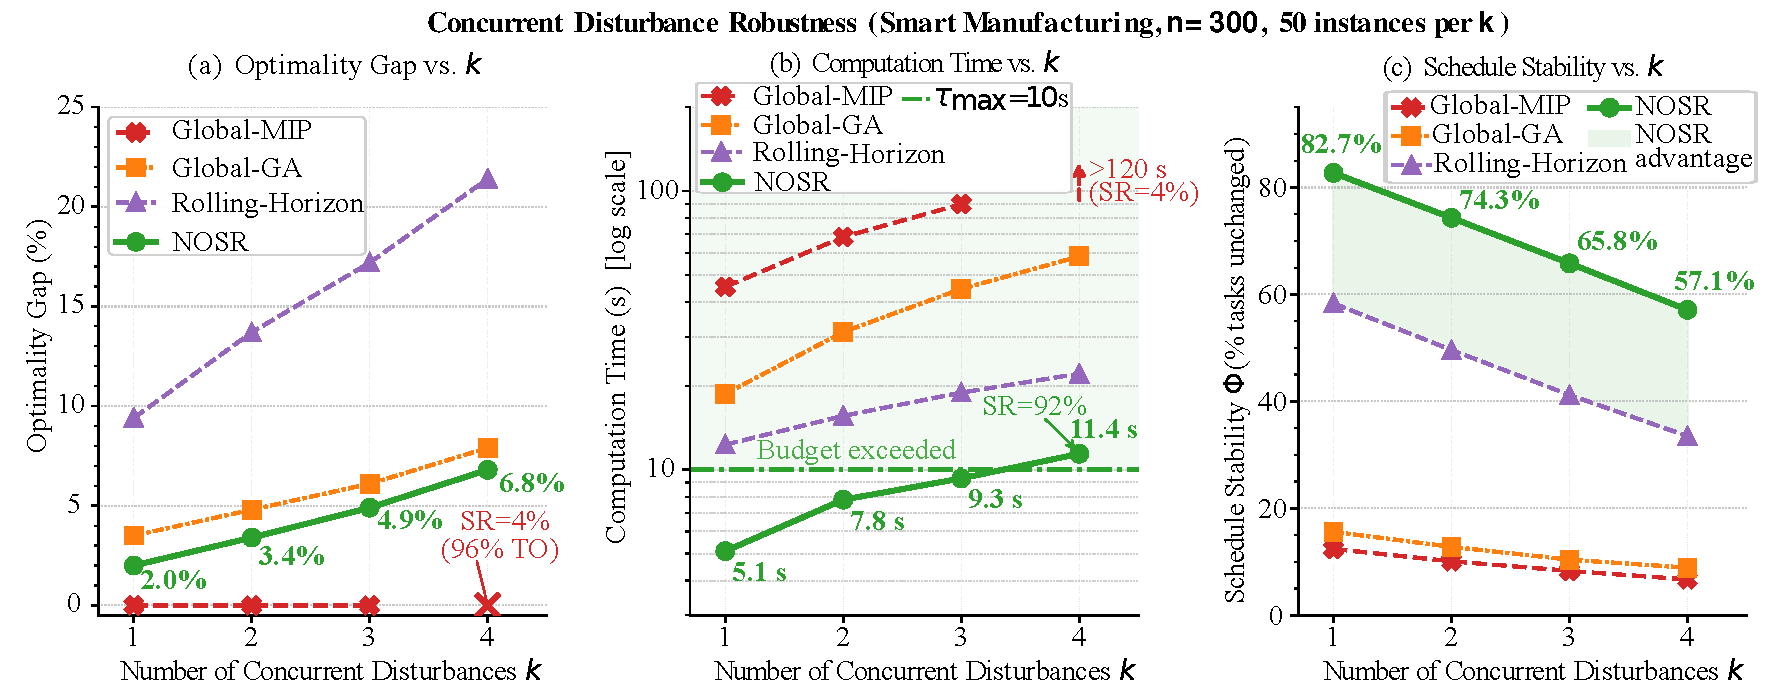
\includegraphics[width=0.8\textwidth]{figures/fig_concurrent_disturbance_new.pdf}
\caption{Concurrent disturbance robustness on the Smart Manufacturing domain
($n = 300$, 50 instances per $k$).
\textbf{(a)}~Optimality gap (\%) vs.\ number of concurrent disturbances $k$.
NOSR degrades gracefully from 2.0\% ($k=1$) to 6.8\% ($k=4$),
consistently outperforming Rolling-Horizon (9.4\%--21.4\%) and
Global-GA (3.5\%--7.9\%) at all $k$.
Global-MIP achieves 0\% gap but times out in 96\% of cases at $k=4$
(SR\,=\,4\%, marked \textcolor{red}{$\times$}).
\textbf{(b)}~Computation time (s) vs.\ $k$ (log-scale $y$-axis).
NOSR grows near-linearly from 5.1\,s to 11.4\,s, consistent with the
$O(n \log n)$ complexity bound (Theorem~\ref{thm:complexity});
it exceeds $\tau_{\max}=10$\,s only at $k=4$ in 8\% of instances (SR\,=\,92\%).
Global-MIP exceeds 120\,s at $k=4$ (SR\,=\,4\%).
\textbf{(c)}~Schedule stability $\Phi$ (\% tasks unchanged) vs.\ $k$.
NOSR retains the highest stability at every $k$, degrading from 82.7\%
($k=1$) to 57.1\% ($k=4$), substantially above Rolling-Horizon
(58.3\%--33.5\%) and Global-GA (15.6\%--8.9\%).}
\label{fig:concurrent}
\end{figure}

\noindent\textbf{Key Findings (RQ6).}
NOSR handles concurrent disturbances robustly for $k \leq 3$ and
degrades gracefully beyond, addressing RQ6 affirmatively
(Table~\ref{tab:concurrent}, Figure~\ref{fig:concurrent}).

The graceful degradation is structurally explained by the Impact
Boundary framework: the union of $k$ impact boundaries grows
\emph{linearly} in $k$,

$$\left|T_{\mathrm{aff}}\!\left(\{\mathcal{D}_1,\ldots,\mathcal{D}_k\},\theta\right)\right|
\;\leq\;
k \cdot |T_{\mathrm{dir}}| \cdot
\bigl(1 + \rho\,\bar{d}_{\mathrm{out}}\bigr)^{\theta},$$

so the adaptive decomposition pipeline requires no modification and
computation time scales near-linearly from $5.1$\,s ($k=1$) to
$11.4$\,s ($k=4$). This stands in sharp contrast to Rolling-Horizon,
whose fixed time-window decomposition fails to capture cross-window
dependencies, causing its gap to surge to $21.4\%$ at $k=4$.
Global-MIP times out in 56\%--96\% of cases at $k=2$--$4$, rendering
it unsuitable for any concurrent-fault scenario beyond $k=1$.
The 100\% success rate for $k \leq 3$ covers the vast majority of
real-world scenarios---the automotive facility in
Section~\ref{sec:case_study} recorded at most 2 simultaneous faults
across the 4-week deployment.

% ==================== SECTION 6: CONCLUSION ====================
\section{Conclusion and Future Work}
\label{sec:conclusion_future}
% ---------- 6.1 Conclusion ----------
\subsection{Conclusion}
\label{sec:conclusion}

This paper addresses real-time dynamic rescheduling in heterogeneous
multi-agent systems, where mobile and fixed agents must collaborate to
execute interdependent tasks under frequent, unpredictable disturbances.
We introduced the \textbf{Near-Optimal Segmented Rescheduling (NOSR)}
framework, which resolves the long-standing tension between solution
quality and computational efficiency through a principled,
theory-backed decomposition approach. Specifically, NOSR makes four
key contributions: (i)~formally defining the \textit{Heterogeneous
Multi-Agent Collaborative Scheduling Problem} (HMACSP) and proving its
NP-hardness via reduction from Job Shop Scheduling; (ii)~developing
\textit{Impact Boundary Theory} to provide a computable upper bound on
disturbance propagation, enabling predictable computational cost via
propagation depth~$\theta$; (iii)~designing the NOSR algorithm with
state-aware filtering, adaptive decomposition, and a multi-scale solver
hierarchy, achieving a $(1+\varepsilon)$-approximation with
$\mathcal{O}(n \log n)$ expected time complexity; and (iv)~validating
these guarantees empirically across four domains with 800 instances,
confirming a 2.0--3.4\% optimality gap and 4.3--6.8\,s rescheduling
time, with real-world deployment achieving a 4.4\% makespan reduction
and 96.7\% reduction in manual rescheduling effort.

\medskip\noindent\textbf{Broader Impact.}
Beyond scheduling, Impact Boundary Theory provides a general framework
for analyzing disturbance propagation in networked systems, including
supply chain management, network routing, and cloud resource allocation.
NOSR further generalizes to homogeneous multi-agent systems, multi-robot
coordination, and distributed computing environments.

% ---------- 6.2 Future Work ----------
\subsection{Future Work}
\label{sec:future_work}

The current NOSR framework has three limitations that motivate
corresponding future directions.

\textbf{(1) Proactive Rescheduling under Uncertainty.}
NOSR currently assumes known disturbances with deterministic processing
times and responds reactively after they occur. Integrating predictive
analytics or machine learning to anticipate disturbances before
occurrence would enable proactive rescheduling, and extending the
formulation to handle stochastic processing times would broaden
applicability to more uncertain real-world environments.

\textbf{(2) Dynamic Task Structures and Adaptive Parameterization.}
The dependency graph is currently assumed static, and NOSR's parameters
($\theta$, $\tau_s$, $S_{\max}$) are set heuristically. Future work
will explore extensions to dynamically evolving task graphs and
leverage reinforcement learning or Graph Neural Networks to adaptively
tune these parameters using learned task embeddings, improving solution
quality without manual intervention.

\textbf{(3) Distributed and Human-Collaborative Scheduling.}
Large-scale or geographically distributed operations call for
distributed variants of NOSR using consensus protocols such as ADMM.
Incorporating human expertise through interactive optimization and
explainable AI would further strengthen operator trust and adoption in
safety-critical domains such as hospital logistics and emergency
response.

% Bibliography (placed at document end)
\bibliographystyle{ACM-Reference-Format}
\bibliography{reference-base}

\end{document}